\documentclass[11pt,a4paper]{article}

% ─── Packages ────────────────────────────────────────────────────────────────
\usepackage[a4paper, margin=2.2cm]{geometry}
\usepackage{booktabs}
\usepackage{longtable}
\usepackage{array}
\usepackage{tabularx}
\usepackage{multirow}
\usepackage{xcolor}
\usepackage{amsmath}
\usepackage{amssymb}
\usepackage{graphicx}
\usepackage{float}
\usepackage{hyperref}
\usepackage{enumitem}
\usepackage{titlesec}
\usepackage{fancyhdr}
\usepackage{parskip}
\usepackage[final,tracking=true,kerning=true,spacing=false,expansion=false]{microtype}
\usepackage[numbers,sort&compress]{natbib}
\usepackage{colortbl}
\usepackage{mdframed}
\usepackage{tikz}
\usetikzlibrary{shapes.geometric, arrows.meta, positioning, fit, backgrounds, calc}

% Make bibliography heading unnumbered
\renewcommand{\refname}{References}
\makeatletter
\renewenvironment{thebibliography}[1]
  {\section*{\refname}%
   \@mkboth{\refname}{\refname}%
   \list{\@biblabel{\@arabic\c@enumiv}}%
        {\settowidth\labelwidth{\@biblabel{#1}}%
         \leftmargin\labelwidth
         \advance\leftmargin\labelsep
         \@openbib@code
         \usecounter{enumiv}%
         \let\p@enumiv\@empty
         \renewcommand\theenumiv{\@arabic\c@enumiv}}%
   \sloppy
   \clubpenalty4000
   \@clubpenalty \clubpenalty
   \widowpenalty4000%
   \sfcode`\.\@m}
  {\def\@noitemerr{\@latex@warning{Empty `thebibliography' environment}}%
   \endlist}
\makeatother

% ─── Colours ─────────────────────────────────────────────────────────────────
\definecolor{sentinelblue}{RGB}{10, 60, 120}
\definecolor{lightgray}{RGB}{245, 245, 245}
\definecolor{rowgray}{RGB}{235, 238, 242}
\definecolor{headerblue}{RGB}{10, 60, 120}
\definecolor{accentorange}{RGB}{210, 95, 30}
\definecolor{successgreen}{RGB}{30, 130, 70}
\definecolor{warningyellow}{RGB}{200, 150, 0}
\definecolor{ersblue}{RGB}{20, 80, 150}
\definecolor{boxbg}{RGB}{240, 245, 255}

% ─── Hyperref ────────────────────────────────────────────────────────────────
\hypersetup{
    colorlinks=true,
    linkcolor=sentinelblue,
    urlcolor=sentinelblue,
    pdftitle={Project Sentinel-BLR v6.1 — Flipkart Gridlock 2.0},
}

% ─── Section formatting ──────────────────────────────────────────────────────
\titleformat{\section}{\large\bfseries\color{sentinelblue}}{\thesection.}{0.7em}{}[\vspace{-0.3em}\rule{\linewidth}{0.4pt}]
\titleformat{\subsection}{\normalsize\bfseries\color{sentinelblue}}{}{0em}{}
\titlespacing{\section}{0pt}{1.4em}{0.6em}
\titlespacing{\subsection}{0pt}{1em}{0.3em}

% ─── Table helpers ───────────────────────────────────────────────────────────
\newcolumntype{L}[1]{>{\raggedright\arraybackslash}p{#1}}
\newcolumntype{C}[1]{>{\centering\arraybackslash}p{#1}}
\renewcommand{\arraystretch}{1.35}

% ─── Callout box ─────────────────────────────────────────────────────────────
\newmdenv[
  backgroundcolor=boxbg,
  linecolor=sentinelblue,
  linewidth=1.5pt,
  leftline=true, rightline=false, topline=false, bottomline=false,
  leftmargin=0pt, rightmargin=0pt,
  innerleftmargin=10pt, innerrightmargin=8pt,
  innertopmargin=6pt, innerbottommargin=6pt,
  skipabove=6pt, skipbelow=6pt
]{callout}

% ─── Header / Footer ─────────────────────────────────────────────────────────
\pagestyle{fancy}
\fancyhf{}
\rhead{\small\color{gray}PROJECT SENTINEL-BLR \textbar\ Flipkart Gridlock 2.0 \textbar\ Phase 2 \textbar\ Theme 3}
\rfoot{\small\color{gray}Sentinel-BLR v6.1 --- Evidence-Quality Traffic Enforcement Framework \textbar\ \thepage}
\renewcommand{\headrulewidth}{0.3pt}
\renewcommand{\footrulewidth}{0.3pt}

% ─────────────────────────────────────────────────────────────────────────────
\begin{document}

% ══════════════════════════════════════════════════════════════════════════════
%  TITLE BLOCK
% ══════════════════════════════════════════════════════════════════════════════
\vspace{1em}
\begin{center}
    {\Huge\bfseries\color{sentinelblue} PROJECT SENTINEL-BLR}\\[0.5em]
    {\large\color{gray} Evidence-Quality Automated Traffic Enforcement Framework}\\[1.2em]
\vspace{2em}
    \begin{tabular}{L{3.5cm} L{11cm}}
        \toprule
        \rowcolor{headerblue}\multicolumn{2}{l}{\color{white}\bfseries Submission Details}\\
        \midrule
        \textbf{Hackathon}       & Flipkart Gridlock 2.0 \\
        \rowcolor{rowgray}
        \textbf{Phase}           & Phase 2 \\
        \textbf{Theme}           & Theme 3 — Automated Photo Identification and Classification for Traffic Violations \\
        \rowcolor{rowgray}
        \textbf{Submission Type} & Framework \& Prototype Proposal \\
        \textbf{Version}         & v6.1 --- Validation \& Trust Pass: Shadow-Mode Phase~1, Conformal ERS Calibration, Citizen Evidence Portal, Synthetic Cold-Start Bootstrap (on the v6.0 Legal \& Cost base) \\
        \rowcolor{rowgray}
        \textbf{Submitted By}    & Team\_Rocket \\
        \bottomrule
    \end{tabular}
\end{center}

\vspace{0.8em}

% ══════════════════════════════════════════════════════════════════════════════
%  AT A GLANCE — ONE-PAGE SKIM SUMMARY
% ══════════════════════════════════════════════════════════════════════════════
\vspace{2em}
\begin{callout}
{\Large\bfseries\color{sentinelblue} Summary at a Glance}\\[0.6em]

\textbf{The idea:} Sentinel-BLR doesn't just detect violations --- it scores how \textit{reliable} each detection is before deciding whether to auto-fine, human-review, or discard it. That score is the \textbf{Evidence Reliability Score (ERS)}, a single 0--100 number combining detection confidence, OCR confidence, multi-frame consensus, calibration health, and image quality.

\vspace{0.4em}
\begin{equation*}
\text{ERS} = 0.30\,C_{\text{det}} + 0.25\,C_{\text{ocr}} + 0.20\,R_{\text{consensus}} + 0.15\,H_{\text{cal}} + 0.10\,Q_{\text{pre}}
\end{equation*}
\vspace{0.2em}

\textbf{Why it matters:} ERS $\geq 85$ $\rightarrow$ auto-fine. 60--84 $\rightarrow$ human review. $<60$ $\rightarrow$ discard, no record. One number replaces five fields for officers and courts --- and structurally prevents a fine being issued on weak evidence.

\textbf{Three structural fixes most pipelines skip:}
\begin{itemize}[leftmargin=1.5em, itemsep=0.15em, topsep=0.2em]
    \item \textbf{Camera drift} --- self-healing Auto-Calibration Heartbeat (SIFT/ORB homography) every 15 min, no enforcement downtime.
    \item \textbf{Unreadable plates} --- 5-frame character-level probability fusion recovers OCR even from mud/rain-damaged plates.
    \item \textbf{Policy as YAML, not model weights} --- BTP can change enforcement rules in $<$1 minute without engineer involvement.
\end{itemize}

\textbf{Cost (Phase 1, 10 junctions):} Edge hardware alone runs in the low lakhs --- Jetson Orin NX modules at $\sim$\$600--970/unit, reusing existing BTP CCTV feeds rather than replacing them. See Section~\ref{sec:layerspec} onward and the Cost and Legal Feasibility section for the full breakdown.

\textbf{Legal grounding (verified, not assumed):} \S129 (helmet), \S128/\S194C (triple riding), \S184(e) (wrong-side --- corrected from an earlier draft's \S185 miscitation), \S194D (repeat-offence escalation), and explicit Digital Personal Data Protection Act 2023 alignment (face-blurring, 24-hour raw-frame deletion). Earlier citation errors were caught and corrected in this version --- see Section~\ref{sec:cost-legal}.

\textbf{Deployment path:} 10 junctions $\rightarrow$ 50 junctions $\rightarrow$ city-wide, each gated by a measurable go/no-go criterion, not a timeline guess.

\textbf{Not a greenfield problem:} Bengaluru's own ITMS, Hyderabad's ANPR e-challan system, and Delhi's RLVD/OSVD network already detect violations at scale. None of them, on current public evidence, score whether a detection is reliable enough to enforce on --- and that gap produced a real 26,000-challan failure in Hyderabad in 2025. See Section~\ref{sec:competitive}.

\vspace{0.3em}
\textbf{What's proven vs.\ what's a design target:} OCR fusion, the calibration heartbeat, and the policy-engine pattern rest on established technique. The $\leq$28~ms standard-condition compute budget and the Volumetric Bounding-Box triple-riding threshold are explicit design targets pending Phase~1 field validation --- and Layer~4A already structurally prevents the least-validated component (triple riding) from ever auto-fining, regardless of confidence. Sentinel-BLR is built to know what it doesn't know yet, not to overclaim certainty it hasn't earned.

\vspace{0.3em}
\vspace{0.3em}
\textbf{How the threshold earns trust (new in this version):} The 85 auto-fine gate is not asserted. Phase~1 runs first in \emph{shadow mode} --- full pipeline, zero fines issued --- so officer adjudications calibrate it (Section~\ref{sec:shadow}); a \emph{conformal} layer then sets per-violation cutoffs carrying a provable $\le$1\% wrongful-fine guarantee (Section~\ref{sec:conformal}); the near-zero local safety labels are bootstrapped by a disciplined \emph{synthetic} pre-training set that real data then replaces (Section~\ref{sec:synthetic}); and every issued challan is contestable through a \emph{citizen evidence portal} whose overturns feed straight back into recalibration (Section~\ref{sec:citizen}).

\vspace{0.3em}
\textbf{Synthetic priors --- data source defined:} Safety-violation count initialisers are absent from the provided datasets (2 helmet and 0 triple-riding records across 298,450 rows in the Police Violations Dataset). Layer~8 initialises violation-type weights to uniform and relies on pre-trained IDD/ACFR/Roboflow Helmet weights as the classification foundation. These priors carry $<$20\% weight from day~1 and are replaced entirely by live field observations within 30 days of Phase~1 operation. They are never used for urgency scoring or auto-fine logic. Section~\ref{sec:synthetic} upgrades these priors into a disciplined synthetic bootstrap training set.

\end{callout}


% ══════════════════════════════════════════════════════════════════════════════
\section{Executive Summary}
% ══════════════════════════════════════════════════════════════════════════════

\textbf{Sentinel-BLR is not a traffic violation detector. It is an evidence-quality system --- one that determines when a detected violation is legally reliable enough for enforcement.}

Most submissions for this problem will bolt together YOLO, OCR, and a violation classifier. Sentinel-BLR does that too --- and then solves the three problems that make those pipelines fail in actual Bengaluru deployment:

\begin{itemize}[leftmargin=1.8em, itemsep=0.3em]
    \item \textbf{Cameras that drift} --- addressed by a self-healing Auto-Calibration Heartbeat (SIFT/ORB + inverse homography $H^{-1}$) detecting and correcting spatial drift every 15 minutes, without halting enforcement.
    \item \textbf{Plates that are unreadable} --- addressed by Temporal Character-Level Probability Fusion across 5 frames with Levenshtein outlier filtering, producing a majority-vote plate string even from mud-damaged plates.
    \item \textbf{Detection confidence that does not translate into legally defensible enforcement} --- addressed by per-violation-type confidence thresholds, a configuration-file policy engine (not an ML model), and a composite Evidence Reliability Score (ERS) on every evidence packet.
\end{itemize}

Sentinel-BLR processes live camera feeds under real-world environmental stress --- night, rain, motion blur, monsoon fog, sodium vapour streetlighting --- and detects all seven categories of traffic violation defined in the problem statement.

\subsection*{Four Architectural Principles}
\begin{enumerate}[leftmargin=1.8em, itemsep=0.2em]
    \item Detect violations reliably under adverse Bengaluru conditions.
    \item Gate enforcement on evidence quality, not raw detection confidence.
    \item Keep all enforcement policy inspectable and updateable without model redeployment.
    \item Produce legally defensible, tamper-evident evidence packets on every confirmed violation.
\end{enumerate}

% ══════════════════════════════════════════════════════════════════════════════
\section{Evidence Reliability Score — The Centrepiece Innovation}
\label{sec:ers}
% ══════════════════════════════════════════════════════════════════════════════

Every other traffic enforcement pipeline asks a single question: \textit{was a violation detected?} Sentinel-BLR asks a second question that no current Indian deployment asks: \textit{is the evidence reliable enough to stand up in enforcement and in court?}

The answer is a single composite integer on every evidence packet --- the \textbf{Evidence Reliability Score (ERS)}. No new model is required; all five input components are computed upstream as part of the standard pipeline.

\subsection*{ERS Formula}

\begin{equation}
\text{ERS} = \underbrace{0.30 \times C_{\text{det}}}_{\text{detection}} + \underbrace{0.25 \times C_{\text{ocr}}}_{\text{plate read}} + \underbrace{0.20 \times R_{\text{consensus}}}_{\text{multi-frame}} + \underbrace{0.15 \times H_{\text{cal}}}_{\text{calibration}} + \underbrace{0.10 \times Q_{\text{pre}}}_{\text{image quality}}
\end{equation}

\noindent All five components are computed upstream as part of the standard pipeline; the ERS introduces no additional inference overhead.

\subsection*{ERS Weight Rationale}

The weights are not arbitrary — they are derived from a failure-consequence hierarchy specific to automated enforcement. Each component is weighted by the severity of the error it guards against:

\begin{center}
\begin{longtable}{L{3.2cm} C{1.2cm} L{9.5cm}}
    \toprule
    \rowcolor{headerblue}
    \color{white}\textbf{Component} & \color{white}\textbf{Weight} & \color{white}\textbf{Rationale} \\
    \midrule
    Detection confidence ($C_{\text{det}}$) & 0.30 & Highest weight: a misclassified violation type (e.g.\ legal manoeuvre flagged as wrong-side) produces a wrongful fine. No downstream check recovers from a wrong detection class. \\
    \rowcolor{rowgray}
    OCR confidence ($C_{\text{ocr}}$) & 0.25 & Second highest: a misread plate issues a fine to the wrong registered owner — a legal liability and a public trust failure. Plate identity is the sole link between evidence and enforcement action. \\
    Frame consensus ($R_{\text{consensus}}$) & 0.20 & A single-frame detection may be a transient artefact (shadow, reflection). Multi-frame agreement is the primary mechanism for suppressing spurious detections; weighted accordingly. \\
    \rowcolor{rowgray}
    Calibration health ($H_{\text{cal}}$) & 0.15 & A drifted camera silently shifts spatial ROIs, producing systematic false positives at stop-lines and parking zones. Important, but recoverable: the heartbeat flags drift and re-projects automatically. \\
    Preprocessing quality ($Q_{\text{pre}}$) & 0.10 & Lowest weight: image degradation affects all upstream components and is already reflected in their confidence scores. This term captures residual uncertainty not absorbed elsewhere (e.g.\ extreme sodium-vapour saturation). \\
    \bottomrule
\end{longtable}
\end{center}

\noindent The top two components together account for 55\% of ERS, directly reflecting that vehicle misidentification and plate misread are the two failure modes most likely to result in a wrongful fine or a successful legal challenge to an enforcement action.

\subsection*{ERS Weight Calibration Status — What Is Claimed and What Is Not}
\vspace{0.3em}
\begin{callout}
The weights (0.30, 0.25, 0.20, 0.15, 0.10) are derived from a \textbf{failure-consequence hierarchy}, not from empirical optimisation on labelled enforcement outcomes. This distinction is stated here deliberately: the hierarchy is logically well-motivated (a misidentified vehicle type cannot be recovered by any downstream check; a misread plate issues a fine to the wrong owner; a single-frame transient differs from a multi-frame event), but the precise numerical values are Phase~1 calibration targets, not validated parameters.

\textbf{Known correlation between components.} $Q_{\text{pre}}$ is not fully independent of $C_{\text{det}}$ and $C_{\text{ocr}}$: severe image degradation depresses all three simultaneously. In practice, the linear formula structurally \emph{amplifies} the penalty for bad-image events --- a low $Q_{\text{pre}}$ frame also yields a lower $C_{\text{det}}$ and $C_{\text{ocr}}$, so the effective ERS penalty from image degradation is larger than the 0.10 weight alone suggests. Section~\ref{sec:ers-casestudy} below quantifies this amplification on a concrete heavy-rain example and explains why it produces a desirable overcaution property rather than a miscalibration.

\textbf{Phase~1 calibration plan.} Every human accept/reject decision in the 60--92\% confidence band generates a labelled outcome. After 500 labelled decisions, a constrained least-squares fit will re-estimate weights subject to the constraint $\sum w_i = 1$, $w_i > 0$. Because $Q_{\text{pre}}$ is partially collinear with $C_{\text{det}}$ and $C_{\text{ocr}}$ (above), the fit is \emph{ridge-regularised} (an L2 penalty on the weight vector): an unregularised least-squares fit on correlated regressors yields unstable, high-variance coefficients, so the regulariser is what keeps the re-estimated weights interpretable rather than an artefact of which collinear term the optimiser happened to load. If the fitted weights diverge from the initial hierarchy by more than $\pm 0.08$ on any component, the ERS formula will be updated and the routing thresholds re-validated before Phase~2 deployment. The initial weights are the prior; live enforcement data provides the posterior. Section~\ref{sec:conformal} adds a conformal calibration layer that bounds the auto-fine error rate directly --- a guarantee that holds \emph{even while} the weights remain an unvalidated prior, because it is a property of the threshold-selection procedure rather than of the weight vector.
\end{callout}

\subsection*{Mock Evidence Packet — What an Enforcement Officer Receives}

The table below illustrates a representative evidence packet output for a helmet non-compliance detection, demonstrating how the ERS translates raw model outputs into a single, actionable enforcement decision:

\begin{longtable}{L{4.5cm} L{9cm}}
    \toprule
    \rowcolor{headerblue}
    \color{white}\textbf{Field} & \color{white}\textbf{Value} \\
    \midrule
    \endfirsthead
    \toprule
    \rowcolor{headerblue}
    \color{white}\textbf{Field} & \color{white}\textbf{Value} \\
    \midrule
    \multicolumn{2}{l}{\small\textit{(continued)}} \\
    \midrule
    \endhead
    \midrule
    \multicolumn{2}{r}{\small\textit{continued on next page}} \\
    \endfoot
    \bottomrule
    \endlastfoot
    Violation Type & Helmet Non-Compliance \\
    \rowcolor{rowgray}
    Vehicle Class & 2-Wheeler \\
    Plate Text & KA~05~MN~4821 \\
    \rowcolor{rowgray}
    OCR Confidence & 94\% (3/5 frames consensus; Levenshtein-clean) \\
    Detection Confidence & 91\% (3-frame consensus; MobileNetV3) \\
    \rowcolor{rowgray}
    Calibration Health & \textcolor{successgreen}{HEALTHY} — last heartbeat 8 min ago, drift 0.3px \\
    Frame Consensus & 5/5 frames in agreement \\
    \rowcolor{rowgray}
    Preprocessing Quality & CLAHE + Retinex active (low-light condition) \\
    SHA-256 Hash & \texttt{3fa2…c91b} (frame tamper-evident) \\
    \rowcolor{rowgray}
    \textbf{Evidence Reliability Score} & \textbf{\textcolor{successgreen}{ERS = 91 / 100 — AUTO-FINE ELIGIBLE}} \\
    MV Act Reference & \S129 (helmet); \S194D enhanced penalty on subsequent offence if repeat offender flagged \\
\end{longtable}

\subsection*{ERS Routing Logic}

\begin{center}
\begin{tabular}{C{2.5cm} L{3.5cm} L{8cm}}
    \toprule
    \rowcolor{headerblue}
    \color{white}\textbf{ERS Range} & \color{white}\textbf{Decision} & \color{white}\textbf{Rationale} \\
    \midrule
    85 – 100 & \textcolor{successgreen}{\textbf{AUTO-FINE}} & All components strong; legally defensible without human review \\
    \rowcolor{rowgray}
    60 – 84  & \textcolor{warningyellow}{\textbf{HUMAN REVIEW}} & One or more components borderline; officer adjudicates \\
    $<$ 60   & \textcolor{red}{\textbf{DISCARD}} & Evidence quality insufficient; no fine, no record \\
    \bottomrule
\end{tabular}
\end{center}

% ══════════════════════════════════════════════════════════════════════════════
\subsection*{ERS in Practice — Three Worked Scenarios and Boundary Sensitivity}
\label{sec:ers-casestudy}
% ══════════════════════════════════════════════════════════════════════════════

The following three scenarios compute ERS end-to-end on representative operating conditions. Component values reflect realistic model outputs under those conditions; the computations demonstrate that ERS routing is fully deterministic and reproducible from five upstream measurements with no additional judgement.

\begin{longtable}{L{4.2cm} C{2.8cm} C{2.8cm} C{2.8cm}}
    \toprule
    \rowcolor{headerblue}
    \color{white}\textbf{Component (weight)} &
    \color{white}\textbf{Scenario A} &
    \color{white}\textbf{Scenario B} &
    \color{white}\textbf{Scenario C} \\
    \midrule
    \endfirsthead
    \toprule
    \rowcolor{headerblue}
    \color{white}\textbf{Component (weight)} &
    \color{white}\textbf{Scenario A} &
    \color{white}\textbf{Scenario B} &
    \color{white}\textbf{Scenario C} \\
    \midrule
    \multicolumn{4}{l}{\small\textit{(continued)}} \\
    \midrule
    \endhead
    \midrule
    \multicolumn{4}{r}{\small\textit{continued on next page}} \\
    \endfoot
    \bottomrule
    \endlastfoot
    \rowcolor{rowgray}
    \multicolumn{4}{l}{\textit{\small Condition}} \\
    & \small Clear day, CLAHE active only & \small Light rain, 3/5 frames usable & \small Heavy rain + damaged plate \\
    \midrule
    $C_{\text{det}}$ --- detection ($\times 0.30$) & 91 & 81 & 62 \\
    \rowcolor{rowgray}
    $C_{\text{ocr}}$ --- plate read ($\times 0.25$) & 94 & 68 & 28 \\
    $R_{\text{consensus}}$ --- multi-frame ($\times 0.20$) & 95 & 75 & 40 \\
    \rowcolor{rowgray}
    $H_{\text{cal}}$ --- calibration ($\times 0.15$) & 100 & 88 & 70 \\
    $Q_{\text{pre}}$ --- image quality ($\times 0.10$) & 85 & 55 & 35 \\
    \midrule
    \textbf{ERS (computed)} & \textbf{93.3} & \textbf{75.0} & \textbf{47.6} \\
    \rowcolor{rowgray}
    \textbf{Routing decision} & \textcolor{successgreen}{\textbf{AUTO-FINE}} & \textcolor{warningyellow}{\textbf{HUMAN REVIEW}} & \textcolor{red}{\textbf{DISCARD}} \\
\end{longtable}

\vspace{0.6em}

\noindent\textbf{Scenario A} (clear day, helmet non-compliance):
\begin{align*}
\text{ERS} &= (0.30 \times 91) + (0.25 \times 94) + (0.20 \times 95) + (0.15 \times 100) + (0.10 \times 85) \\
           &= 27.3 + 23.5 + 19.0 + 15.0 + 8.5 \;=\; \mathbf{93.3} \;\rightarrow\; \textcolor{successgreen}{\text{AUTO-FINE}}
\end{align*}

\noindent\textbf{Scenario B} (light rain, partial plate occlusion):
\begin{align*}
\text{ERS} &= (0.30 \times 81) + (0.25 \times 68) + (0.20 \times 75) + (0.15 \times 88) + (0.10 \times 55) \\
           &= 24.3 + 17.0 + 15.0 + 13.2 + 5.5 \;=\; \mathbf{75.0} \;\rightarrow\; \textcolor{warningyellow}{\text{HUMAN REVIEW}}
\end{align*}

\noindent\textbf{Scenario C} (heavy rain, mud-damaged plate):
\begin{align*}
\text{ERS} &= (0.30 \times 62) + (0.25 \times 28) + (0.20 \times 40) + (0.15 \times 70) + (0.10 \times 35) \\
           &= 18.6 + 7.0 + 8.0 + 10.5 + 3.5 \;=\; \mathbf{47.6} \;\rightarrow\; \textcolor{red}{\text{DISCARD}}
\end{align*}

\subsubsection*{Boundary Sensitivity — What Changes at ERS = 84 vs.\ 85?}

The boundary between AUTO-FINE and HUMAN REVIEW is the decision point with the largest enforcement consequence. The scenario below constructs a case sitting just below the 85 threshold and analyses what would happen under two alternative policy choices.

\textbf{Boundary scenario} (marginal detection, calibration drift approaching limit):
\begin{itemize}[leftmargin=1.8em, itemsep=0.15em]
    \item $C_{\text{det}} = 88$ (detection confident, 3-frame consensus met)
    \item $C_{\text{ocr}} = 91$ (plate read confirmed, Levenshtein-clean)
    \item $R_{\text{consensus}} = 80$ (3/5 frames, not 5/5 — two frames motion-blurred)
    \item $H_{\text{cal}} = 78$ (calibration heartbeat 13~min ago, drift 1.1~px — approaching the 1.2~px alert threshold)
    \item $Q_{\text{pre}} = 65$ (CLAHE + Retinex active, moderate sodium-vapour distortion)
\end{itemize}

\begin{align*}
\text{ERS} &= (0.30 \times 88) + (0.25 \times 91) + (0.20 \times 80) + (0.15 \times 78) + (0.10 \times 65) \\
           &= 26.4 + 22.75 + 16.0 + 11.7 + 6.5 \;=\; \mathbf{83.35} \;\rightarrow\; \textcolor{warningyellow}{\text{HUMAN REVIEW}} \checkmark
\end{align*}

\begin{longtable}{L{5cm} C{2.5cm} C{2.5cm} L{4cm}}
    \toprule
    \rowcolor{headerblue}
    \color{white}\textbf{Policy variant} & \color{white}\textbf{ERS} & \color{white}\textbf{Decision} & \color{white}\textbf{Risk implication} \\
    \midrule
    \endfirsthead
    \toprule
    \rowcolor{headerblue}
    \color{white}\textbf{Policy variant} & \color{white}\textbf{ERS} & \color{white}\textbf{Decision} & \color{white}\textbf{Risk implication} \\
    \midrule
    \multicolumn{4}{l}{\small\textit{(continued)}} \\
    \midrule
    \endhead
    \midrule
    \multicolumn{4}{r}{\small\textit{continued on next page}} \\
    \endfoot
    \bottomrule
    \endlastfoot
    Baseline (threshold = 85) & 83.35 & \textcolor{warningyellow}{\textbf{REVIEW}} & Officer adjudicates; no wrongful fine \\
    \rowcolor{rowgray}
    Threshold lowered to 80 & 83.35 & \textcolor{red}{\textbf{AUTO-FINE}} & Camera drift at 1.1~px + motion blur = exactly Hyderabad's reported sync-failure mode; auto-fine would issue \\
    OCR weight shifted to 0.20 (redistributed to $R_{\text{consensus}}$ 0.25) & 82.8 & \textcolor{warningyellow}{\textbf{REVIEW}} & Same decision; delta = $-0.55$. This packet sits 1.65 below the gate, so a $\pm$0.05 weight shift ($\approx\pm$0.55 ERS) cannot flip it. Stability exactly at the 84/85 boundary is a Phase~1 calibration check, not claimed from this case \\
    \rowcolor{rowgray}
    OCR weight shifted to 0.30 (redistributed from $R_{\text{consensus}}$ 0.20 to 0.15) & 83.9 & \textcolor{warningyellow}{\textbf{REVIEW}} & Delta = $+0.55$; still REVIEW \\
\end{longtable}

\vspace{0.5em}

\noindent\textbf{Why the 85 threshold holds for this case.} $H_{\text{cal}} = 78$ signals a camera approaching its drift alert boundary. A routing policy that auto-fined this packet would replicate the failure mode documented in Hyderabad's 26,000-challan episode: a weak individual signal ($H_{\text{cal}}$ borderline, $R_{\text{consensus}}$ at 80 not 95) passing through a threshold set too low. The 85 boundary ensures that \emph{no single strong component can carry a weak packet to auto-fine}: even with $C_{\text{det}} = 88$ and $C_{\text{ocr}} = 91$, the borderline calibration and incomplete consensus pull ERS below the gate.

\subsubsection*{The $Q_{\text{pre}}$ Correlation Effect — A Feature, Not a Flaw}

In Scenario~C ($Q_{\text{pre}} = 35$), severe image degradation does not merely subtract $0.10 \times (85 - 35) = 5.0$ points from ERS. It simultaneously depresses $C_{\text{det}}$ by approximately 29 points and $C_{\text{ocr}}$ by approximately 66 points relative to clear-condition baselines. The total ERS impact of image degradation in Scenario~C:

\begin{align*}
\text{Direct } Q_{\text{pre}} \text{ penalty:}& \quad 0.10 \times (85 - 35) = 5.0 \text{ points} \\
\text{Cascaded via } C_{\text{det}}:& \quad 0.30 \times (91 - 62) = 8.7 \text{ points} \\
\text{Cascaded via } C_{\text{ocr}}:& \quad 0.25 \times (94 - 28) = 16.5 \text{ points} \\
\textbf{Total degradation impact:}& \quad \mathbf{30.2 \text{ points}} \text{ vs.\ 5.0 from } Q_{\text{pre}} \text{ alone}
\end{align*}

This amplification means any severe-image-quality event drives ERS well below 60 regardless of what the detection model reports --- a structurally desirable property. Mud on a lens, heavy monsoon rain, or extreme sodium-vapour saturation produces DISCARD outcomes rather than borderline HUMAN REVIEW outcomes that might produce inconsistent officer adjudication. Phase~1 will measure whether this amplification is appropriately calibrated or creates an overcaution bias in specific lighting conditions (e.g.\ moderate rain that degrades OCR but leaves detection reliable).

% ══════════════════════════════════════════════════════════════════════════════
% ══════════════════════════════════════════════════════════════════════════════
\section{Conformal Calibration of the ERS — From a Hand-Set Threshold to a Guaranteed Error Rate}
\label{sec:conformal}
% ══════════════════════════════════════════════════════════════════════════════

\noindent The ERS section is deliberately honest that the weights ($0.30, 0.25, \dots$) and the 85 auto-fine threshold are a \emph{logically-motivated prior}, not parameters validated against enforcement outcomes (Section~\ref{sec:ers}). The ridge-regularised re-fit described there improves the \emph{weights}, but it still leaves the question a deploying agency actually cares about unanswered: \textit{when Sentinel-BLR auto-fines, how often is it wrong?} A weight vector does not answer that; a calibrated threshold does. This section adds the layer that converts the 85 cutoff from an asserted number into one carrying a distribution-free statistical guarantee.

\subsection*{The Idea — Conformal Risk Control on the Auto-Fine Region}

Conformal prediction is a distribution-free wrapper that turns a model's score into a decision carrying a \emph{finite-sample, assumption-light error guarantee} \cite{angelopoulos2023conformal, vovk2005alrw}. Applied to ERS, it works as follows. Let the target wrongful-auto-fine rate be $\alpha$ (e.g.\ $\alpha = 0.01$: at most 1\% of auto-fines may be erroneous). From shadow-mode operation (Section~\ref{sec:shadow}) we obtain a calibration set of $n$ events the pipeline \emph{wanted} to auto-fine, each with an officer-adjudicated ground-truth label (\textsc{correct} / \textsc{wrongful}). Define, on that calibration set, the empirical wrongful-fine rate above a candidate threshold $t$:

\begin{equation}
\widehat{R}(t) = \frac{\#\{\, i : \text{ERS}_i \ge t \ \wedge\ \text{label}_i = \textsc{wrongful} \,\}}{\#\{\, i : \text{ERS}_i \ge t \,\}}.
\end{equation}

Conformal risk control \cite{angelopoulos2024crc} then selects the \emph{lowest} threshold whose risk, inflated by a finite-sample slack $\hat{\lambda}(n,\delta)$, still meets the target:

\begin{equation}
\text{ERS}^{\star} = \min\big\{\, t : \widehat{R}(t) + \hat{\lambda}(n,\delta) \le \alpha \,\big\}.
\end{equation}

Auto-fine is permitted only when $\text{ERS}_i \ge \text{ERS}^{\star}$. Under exchangeability of the calibration and live streams, this construction guarantees, with confidence $1-\delta$, that the wrongful-auto-fine rate inside the auto-fine region is bounded by $\alpha$ --- \emph{regardless of whether the ERS weights are optimal}. The guarantee is a property of the calibration procedure, not of the weight vector, which is exactly why it survives the proposal's own admission that the weights are an unvalidated prior.

\subsection*{Per-Violation-Type Calibration (Mondrian Conformal)}

A single global cutoff hides that the seven violation types have very different error profiles --- helmet detection on a clear plate is not wrong-side inference from contested OSM geometry. Sentinel-BLR therefore calibrates \emph{class-conditionally} (Mondrian conformal): each violation type gets its own $\text{ERS}^{\star}_{\text{type}}$, computed only from that type's calibration labels. The single global 85 of Section~\ref{sec:ers} becomes a per-type vector that the \emph{data} sets, not an engineer. Illustrative cutoffs at $\alpha = 0.01$ (to be replaced by shadow-mode-measured values):

\begin{center}
\begin{tabular}{L{3.4cm} C{2.6cm} C{3.0cm} L{4.6cm}}
    \toprule
    \rowcolor{headerblue}
    \color{white}\textbf{Violation type} & \color{white}\textbf{Hand-set gate (v6.0)} & \color{white}\textbf{Conformal $\text{ERS}^{\star}$ (illustrative)} & \color{white}\textbf{Effect} \\
    \midrule
    Helmet & 85 & 86 & $\approx$ unchanged; clean signal \\
    \rowcolor{rowgray}
    Stop-line / red-light & 85 & 88 & Raised; signal-state coupling risk \\
    Wrong-side driving & 85 & 92 & Raised sharply; contested geometry \\
    \rowcolor{rowgray}
    Illegal parking & 85 & 84 & Lowered slightly; duration adds evidence \\
    Triple riding & \multicolumn{2}{c}{never auto-fine} & Human review only (unchanged) \\
    \rowcolor{rowgray}
    Seatbelt (Phase 1) & \multicolumn{2}{c}{never auto-fine} & Human review only (unchanged) \\
    \bottomrule
\end{tabular}
\end{center}

\noindent The hardest categories \emph{automatically} demand a higher ERS to auto-fine, with no per-type hand-tuning --- the calibration data raises the bar exactly where the error risk is highest.

\subsection*{Where It Sits, and What Breaks It (Honest Scoping)}

The conformal layer sits between Layer~4 (confidence gate) and Layer~4A (policy engine): it does not replace the ERS, it calibrates the cutoff the policy engine enforces. Three honest limits:

\begin{itemize}[leftmargin=1.8em, itemsep=0.25em]
    \item \textbf{Exchangeability is an assumption, and drift violates it.} A camera that drifts or a monsoon that shifts the image distribution breaks the i.i.d.-like condition the guarantee rests on. Mitigation: cutoffs are recomputed on a rolling calibration window, and any distribution-shift alarm --- the Layer~1A calibration heartbeat or a data-drift monitor --- invalidates the current cutoff and reverts that junction to the conservative fixed gate plus human review until re-calibrated.
    \item \textbf{It needs labels.} A few hundred adjudicated outcomes \emph{per type} are required before a per-type guarantee is meaningful. Until shadow mode supplies them, the system falls back to the fixed 85 gate and routes aggressively to human review. Rare classes (triple riding, wrong-side) may never accumulate enough auto-fine-candidate labels --- which is consistent with, not contrary to, their existing human-review-only status.
    \item \textbf{It bounds one error, not all.} Conformal risk control here bounds the \emph{wrongful-fine} (false-positive) rate --- the politically and legally costly direction. Missed violations (recall) are governed separately by the per-type recall targets in Section~\ref{sec:eval}.
\end{itemize}

\noindent The pitch is therefore precise. \textbf{Sentinel-BLR does not ask BTP to trust a hand-set 85. It auto-fines only inside a region whose wrongful-fine rate is provably $\le 1\%$ at 95\% confidence, with the threshold set by data, re-validated against drift, and falling back to human review whenever the guarantee cannot be supported.}

% ══════════════════════════════════════════════════════════════════════════════
\section{System at a Glance — Naive Approach vs.\ Sentinel-BLR}
\label{sec:naive-vs-sentinel}
% ══════════════════════════════════════════════════════════════════════════════

The pipeline comparison below illustrates, at each processing stage, the structural gap between a standard YOLO+OCR approach and the Sentinel-BLR evidence-quality framework. Each layer on the right directly addresses a documented failure mode of the left.

\vspace{0.8em}

% ─── TikZ Side-by-Side Pipeline ──────────────────────────────────────────────
\begin{figure}[H]
\centering
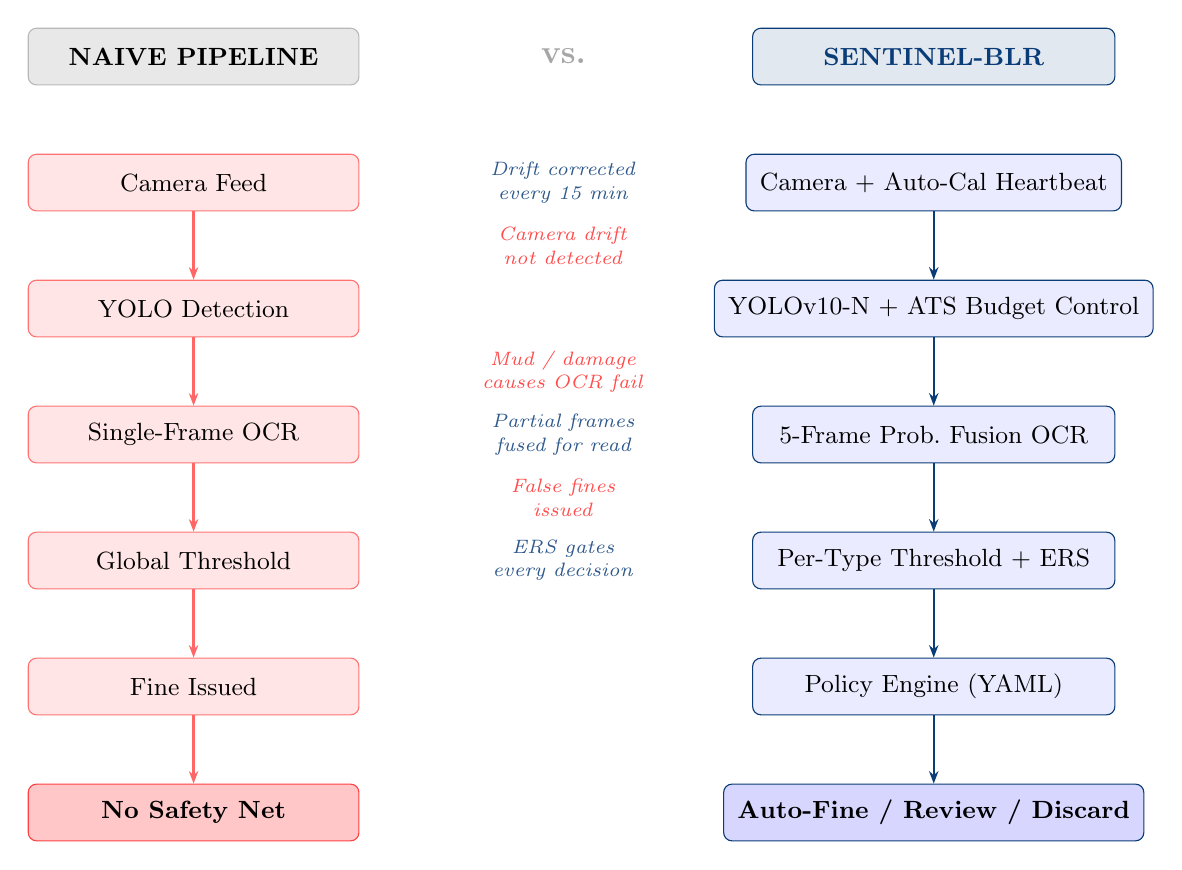
\begin{tikzpicture}[
    naivebox/.style={rectangle, rounded corners=3pt,
        minimum width=4.2cm, minimum height=0.72cm,
        text centered, font=\small, inner sep=5pt,
        fill=red!10, draw=red!55},
    sentbox/.style={rectangle, rounded corners=3pt,
        minimum width=4.6cm, minimum height=0.72cm,
        text centered, font=\small, inner sep=5pt,
        fill=blue!8, draw=sentinelblue},
    labelbox/.style={rectangle, rounded corners=3pt,
        minimum width=4.2cm, minimum height=0.72cm,
        text centered, font=\small\bfseries, inner sep=5pt,
        fill=gray!18, draw=gray!55},
    sentlabel/.style={rectangle, rounded corners=3pt,
        minimum width=4.6cm, minimum height=0.72cm,
        text centered, font=\small\bfseries, inner sep=5pt,
        fill=sentinelblue!12, draw=sentinelblue},
    badbox/.style={rectangle, rounded corners=3pt,
        minimum width=4.2cm, minimum height=0.72cm,
        text centered, font=\small, inner sep=5pt,
        fill=red!22, draw=red!75},
    goodbox/.style={rectangle, rounded corners=3pt,
        minimum width=4.6cm, minimum height=0.72cm,
        text centered, font=\small, inner sep=5pt,
        fill=blue!16, draw=sentinelblue},
    narrow/.style={-{Stealth[length=4.5pt]}, thick, color=red!60},
    sarrow/.style={-{Stealth[length=4.5pt]}, thick, color=sentinelblue},
    failnote/.style={font=\fontsize{7}{8.5}\selectfont\itshape,
        text=red!70, align=center, text width=2.2cm},
    fixnote/.style={font=\fontsize{7}{8.5}\selectfont\itshape,
        text=sentinelblue!85, align=center, text width=2.4cm},
]

% ── LEFT PIPELINE (centred at x=0) ──────────────────────────────────────────
\node[labelbox]   at (0,    0)    (nl) {NAIVE PIPELINE};
\node[naivebox]   at (0,  -1.6)   (n1) {Camera Feed};
\node[naivebox]   at (0,  -3.2)   (n2) {YOLO Detection};
\node[naivebox]   at (0,  -4.8)   (n3) {Single-Frame OCR};
\node[naivebox]   at (0,  -6.4)   (n4) {Global Threshold};
\node[naivebox]   at (0,  -8.0)   (n5) {Fine Issued};
\node[badbox]     at (0,  -9.6)   (n6) {\textbf{No Safety Net}};

\draw[narrow] (n1.south) -- (n2.north);
\draw[narrow] (n2.south) -- (n3.north);
\draw[narrow] (n3.south) -- (n4.north);
\draw[narrow] (n4.south) -- (n5.north);
\draw[narrow] (n5.south) -- (n6.north);

% ── RIGHT PIPELINE (centred at x=9.4) ───────────────────────────────────────
\node[sentlabel]  at (9.4,  0)    (sl) {\color{sentinelblue}SENTINEL-BLR};
\node[sentbox]    at (9.4, -1.6)  (s1) {Camera + Auto-Cal Heartbeat};
\node[sentbox]    at (9.4, -3.2)  (s2) {YOLOv10-N + ATS Budget Control};
\node[sentbox]    at (9.4, -4.8)  (s3) {5-Frame Prob.\ Fusion OCR};
\node[sentbox]    at (9.4, -6.4)  (s4) {Per-Type Threshold + ERS};
\node[sentbox]    at (9.4, -8.0)  (s5) {Policy Engine (YAML)};
\node[goodbox]    at (9.4, -9.6)  (s6) {\textbf{Auto-Fine / Review / Discard}};

\draw[sarrow] (s1.south) -- (s2.north);
\draw[sarrow] (s2.south) -- (s3.north);
\draw[sarrow] (s3.south) -- (s4.north);
\draw[sarrow] (s4.south) -- (s5.north);
\draw[sarrow] (s5.south) -- (s6.north);

% ── VS LABEL ────────────────────────────────────────────────────────────────
\node[font=\large\bfseries, text=gray!70] at (4.7, 0) {vs.};

% ── ANNOTATIONS (centred in the gap between columns) ────────────────────────
% Each annotation sits at mid-x=4.7, at the y of the relevant row.
% Failure notes (red) above fix notes (blue) where both apply.

\node[failnote] at (4.7, -2.4)  {Camera drift\\not detected};
\node[fixnote]  at (4.7, -1.6)  {Drift corrected\\every 15 min};

\node[failnote] at (4.7, -4.0)  {Mud / damage\\causes OCR fail};
\node[fixnote]  at (4.7, -4.8)  {Partial frames\\fused for read};

\node[failnote] at (4.7, -5.6)  {False fines\\issued};
\node[fixnote]  at (4.7, -6.4)  {ERS gates\\every decision};

\end{tikzpicture}
\caption{Standard YOLO+OCR pipeline (left) vs.\ Sentinel-BLR evidence-quality pipeline (right). Red annotations mark naive failure modes; blue annotations indicate the corresponding Sentinel-BLR mitigation.}
\label{fig:naive-vs-sentinel}
\end{figure}
% ─────────────────────────────────────────────────────────────────────────────

\vspace{0.5em}

\begin{longtable}{L{3.2cm} L{4.5cm} L{7cm}}
    \toprule
    \rowcolor{headerblue}
    \color{white}\textbf{Problem} & \color{white}\textbf{Naive Approach} & \color{white}\textbf{Sentinel-BLR v6.1} \\
    \midrule
    \endfirsthead
    \toprule
    \rowcolor{headerblue}
    \color{white}\textbf{Problem} & \color{white}\textbf{Naive Approach} & \color{white}\textbf{Sentinel-BLR v6.1} \\
    \midrule
    \endhead
    \bottomrule
    \endfoot

    Camera drift & Manual recalibration & Auto-Calibration Heartbeat (SIFT/ORB + $H^{-1}$ ROI re-projection) every 15~min \\
    \rowcolor{rowgray}
    Dirty / occluded plates & Single-frame OCR & Temporal Character-Level Probability Fusion across 5 frames + Levenshtein outlier filter \\
    Dense traffic triple riding & Pose estimation (fails in crowds) & Volumetric Bounding-Box Profiling (primary, crowd index $> 0.35$); MediaPipe Pose Lite (enhancement, index $\leq 0.35$); 3-frame consensus \\
    \rowcolor{rowgray}
    False automated fines & Global confidence threshold & Per-violation thresholds + Layer~4A YAML policy engine + ERS; OCR confirmation required \\
    Compute feasibility & Theoretical benchmark & ATS + TensorRT INT8 $\rightarrow$ $\leq$28~ms standard / $\leq$38~ms adverse-peak design target on Jetson Orin NX (see compute budget note in Section~\ref{sec:layerspec}) \\
    \rowcolor{rowgray}
    Kafka bandwidth & Raw frame streaming & Hybrid Evidence Payload: JSON + ROI JPEG crop ($<$50~KB) \\
    Safety violation data scarcity & Zero-initialise or ignore & Uniform priors (safety violations are absent from provided datasets) + pre-trained IDD/ACFR/Roboflow Helmet weights as classification foundation; live data dominates after 30 days \\
\end{longtable}

% ══════════════════════════════════════════════════════════════════════════════
\section{Competitive Landscape — What Already Runs on Bengaluru's Roads}
\label{sec:competitive}
% ══════════════════════════════════════════════════════════════════════════════

This is not a greenfield problem, and treating it as one would undersell what Sentinel-BLR actually contributes. Bengaluru already operates an AI-based enforcement system, and at least two other major Indian metros run comparable infrastructure at larger scale. The naive pipeline in Section~\ref{sec:naive-vs-sentinel} is a pedagogical baseline, not a claim that no automated system exists today --- the comparison that actually matters is against what BTP and peer cities have deployed, what they say it does, and what has gone wrong with it in practice.

\subsection*{What's Already Deployed}

\begin{longtable}{L{3.3cm} L{5.8cm} L{6.2cm}}
    \toprule
    \rowcolor{headerblue}
    \color{white}\textbf{City / System} & \color{white}\textbf{Stated Capability} & \color{white}\textbf{Documented Gap} \\
    \midrule
    \endfirsthead
    \toprule
    \rowcolor{headerblue}
    \color{white}\textbf{City / System} & \color{white}\textbf{Stated Capability} & \color{white}\textbf{Documented Gap} \\
    \midrule
    \endhead
    \bottomrule
    \endfoot

    Bengaluru --- ITMS (live since Dec~2022) & 250 ANPR cameras + 80 red-light violation cameras across 50 junctions; stated to detect speeding, red-light/stop-lane, helmetless riding, triple riding, mobile-phone use, and seatbelt non-compliance~\cite{btpitms2023} & BTP's own Joint Commissioner of Police (Traffic) stated in 2024 that ITMS does not detect violations including wrong-side driving and footpath riding, and that registering such cases from CCTV footage ``is a manual process'' --- prompting a renewed physical-enforcement drive for exactly the violation categories this problem statement lists~\cite{btpanucheth2024} \\
    \rowcolor{rowgray}
    Hyderabad / Cyberabad --- ANPR e-challan (since 2018) & City-wide ANPR plus violation-classifier pipeline issuing automated challans for overspeeding, signal jumping, helmet, and seatbelt offences~\cite{hyderabadanpr2018} & In the first ten months of 2025, the Cyberabad, Hyderabad, and Rachakonda commissionerates together issued over 26,000 wrong challans. Officials attributed the bulk of these to the violation-detection system and the plate-reading system falling out of sync with each other, including challans issued to vehicles in unrelated parts of the city~\cite{hyderabadwrongchallan2025} \\
    Delhi --- ITMS / RLVD--OSVD & 334 radar-based Red-Light Violation Detection and Over-Speed Violation Detection cameras installed, with 328 more under procurement, as part of an AI-based ITMS monitoring movement, violations, and accidents~\cite{delhiitms2026} & Public reporting on the programme centres on camera counts and procurement timelines, not on plate-OCR accuracy, evidence-reliability scoring, or auto-fine precision under adverse conditions --- the specific questions this problem statement and Sentinel-BLR are built to answer \\
\end{longtable}

\subsection*{Why This Reframes Sentinel-BLR's Contribution}

Two conclusions follow directly from the table above, and both sharpen rather than weaken the pitch.

\noindent\textbf{First, Bengaluru does not need another violation detector --- it needs the layer its own system is missing.} BTP has already stated, on record, which violation categories its existing AI infrastructure cannot yet automate safely: wrong-side driving and footpath/lane violations, both disproportionately exposed to false positives, where a wrong call is a wrongful fine rather than merely a missed one. Sentinel-BLR is not positioned as a replacement for ITMS's 250 ANPR and 80 RLVD cameras. It is positioned as the evidence-reliability layer --- ERS (Section~\ref{sec:ers}), per-violation confidence gating, and the Layer~4A policy engine --- that would let BTP extend automated enforcement into precisely the categories it has publicly said it cannot yet trust to a machine, without having to re-architect the camera network it has already paid for.

\noindent\textbf{Second, Hyderabad's 2025 wrong-challan episode is not a hypothetical risk invented for this proposal --- it already happened, at comparable scale, on a comparable architecture.} A detection model and an OCR model running independently and silently drifting out of sync is exactly the failure mode that issues a fine to the wrong vehicle. This is precisely what Layer~5's temporal character-level probability fusion and the ERS's 0.25 weight on OCR confidence exist to prevent: no auto-fine is issued unless plate identity \emph{and} violation detection are jointly confident, not separately plausible and independently wrong. Where Hyderabad's reported failure mode comes from treating detection and OCR as two systems that happen to agree, Sentinel-BLR treats their joint reliability as the enforcement decision itself.

The honest claim is therefore not ``no one has built AI traffic enforcement in Indian cities before.'' It is: \textbf{deployed systems already detect violations; none of them, on current public evidence, structurally score whether that detection is reliable enough to enforce on} --- and the absence of that layer has already produced a real, reported, 26,000-challan failure in a comparable city deployment. Sentinel-BLR's central innovation exists for a failure mode that has already occurred elsewhere, not a theoretical one.

% ══════════════════════════════════════════════════════════════════════════════
\section{System Architecture — Full Pipeline v6.1}
% ══════════════════════════════════════════════════════════════════════════════

The pipeline processes camera feeds through fifteen distinct layers, each with a defined responsibility and explicit computational budget. Detection and enforcement are deliberately separated: Layer~3 detects; Layer~4A applies enforcement policy as a configuration file, not an ML model.

Three Evidence-Quality Layers --- Layer~1A (auto-calibration), Layer~2A (inference budget controller + ATS), and Layer~4A (enforcement policy engine) --- together constitute the architecture's spine.
\subsection*{Pipeline Architecture Diagram}

\begin{figure}[H]
            \centering
            
\includegraphics[width=0.70\linewidth]{Layer 2 Macro Detection YOLOv10-N Tensor INT8 ByteTrack 11 Classes (5).png}
            \label{fig:placeholder}
        \caption{Sentinel-BLR Full System Architecture}
    \label{fig:architecture}
\end{figure}

\newpage
\subsection*{Layer Reference Table}

\begin{longtable}{C{1.2cm} L{3cm} L{6.8cm} L{2.5cm}}
    \toprule
    \rowcolor{headerblue}
    \color{white}\textbf{Layer} & \color{white}\textbf{Function} & \color{white}\textbf{Technical Detail} & \color{white}\textbf{Group} \\
    \midrule
    \endfirsthead
    \toprule
    \rowcolor{headerblue}
    \color{white}\textbf{Layer} & \color{white}\textbf{Function} & \color{white}\textbf{Technical Detail} & \color{white}\textbf{Group} \\
    \midrule
    \endhead
    \bottomrule
    \endfoot

    0 & Feed Ingestion & RTSP/ONVIF camera streams; edge-local ring buffer; Kafka Hybrid Evidence Payloads (JSON + ROI JPEG); dynamic 5–30~fps per junction & INGESTION \\
    \rowcolor{rowgray}
    1 & Environmental Preprocessing & CLAHE, Multi-Scale Retinex, DCP de-hazing, Wiener de-blur; GPU-accelerated; conditionally activated per frame & PREPROC \\
    \textcolor{accentorange}{\textbf{1A $\bigstar$}} & Auto-Calibration Heartbeat & SIFT/ORB landmark extraction every 15~min; homography $H$; drift alert $> 1.2$~px; inverse $H^{-1}$ re-projects all spatial ROIs automatically & PREPROC \\
    \rowcolor{rowgray}
    2 & Macro Detection & YOLOv10-N TensorRT INT8 at 640px ($\sim$4–7~ms); ByteTrack edge-local; 11 classes & DETECTION \\
    \textcolor{accentorange}{\textbf{2A $\bigstar$}} & Inference Budget Controller + ATS & Trigger-gated sub-model activation; async priority queues; per-Track-ID gating (0.5s window); Adaptive Temporal Striding (every 5th frame in adverse weather) & DETECTION \\
    \rowcolor{rowgray}
    3 & Violation Detection Engine & 5 parallel triggered paths: (A) Helmet/Seatbelt, (B) Triple Riding hybrid, (C) Wrong-Side, (D) Stop-Line/Red-Light, (E) Illegal Parking & CLASSIF. \\
    4 & Confidence Gate & Per-violation-type multi-frame consensus thresholds; three-way escalation router: AUTO-FINE / HUMAN REVIEW / DISCARD & DECISION \\
    \rowcolor{rowgray}
    \textcolor{accentorange}{\textbf{4A $\bigstar$}} & Enforcement Policy Engine & YAML config file (not ML); BTP-updatable in $<$1~min; graduated warning tier; diversion polygon support; OCR-gate and calibration-gate enforcement rules & DECISION \\
    5 & License Plate OCR & PaddleOCR PP-OCRv4; Temporal Character-Level Probability Fusion (5-frame softmax sum + argmax); Levenshtein outlier filter; KA-regex gate & ID \\
    \rowcolor{rowgray}
    5A & Repeat Offender Tracking & Cross-junction plate-violation index; 24h/7d/30d lookback; REPEAT OFFENDER flag; enhanced subsequent-offence penalties under MV Act 2019 \S194C/\S194D; HIGH CONFIDENCE writes only & ID \\
    6A & GradCAM Explainability & Saliency overlay on all flagged frames; async low-priority queue (no pipeline latency); legal defensibility and active learning & EVIDENCE \\
    \rowcolor{rowgray}
    6 & Evidence Packet Generator & Annotated frame + GradCAM + UTC + GPS + junction ID + plate + violation type + vehicle class + SHA-256 + \textbf{ERS (0–100)} & EVIDENCE \\
    7 & Persistence & PostgreSQL + TimescaleDB; DuckDB batch analytics; nightly 02:00 aggregation & STORAGE \\
    \rowcolor{rowgray}
    8 & Strategic Intelligence & Junction Urgency Score; recency-decay $0.95^{\text{days}}$; synthetic priors $<$20\% weight after 30 days; weekly LoRA fine-tuning & INTEL \\
    9 & Analytics Dashboard & GIS Live Map; Junction Heatmap; Peak-Hour Trends; Human Review Queue; Deployment Recommendations; Model Performance; Calibration Health; Public Compliance Feed & OUTPUT \\
\end{longtable}

% ══════════════════════════════════════════════════════════════════════════════
\section{The Six Key Differentiators}
% ══════════════════════════════════════════════════════════════════════════════

\noindent The six properties below are what separate Sentinel-BLR from a standard YOLO+OCR assembly. Each is a direct response to a documented failure mode; full technical specification appears in Section~\ref{sec:layerspec}. Three of the six (character-level OCR fusion, the calibration heartbeat, and policy-as-config) rest on established technique. The remaining three (ATS, the compute budget, and the triple-riding hybrid) are explicit design targets gated behind Phase~1 field validation --- and the policy engine in Layer~4A is deliberately structured so that the least-validated component, triple riding, can never auto-fine regardless of confidence. The system is designed to be honest about its own uncertainty rather than to assume it away.

\begin{enumerate}[leftmargin=1.8em, itemsep=0.6em]

    \item \textbf{Adaptive Temporal Striding (ATS) — degradation without coverage loss.}
    Most systems suppress sub-models under adverse weather, silently dropping violation coverage. ATS instead processes every 5th frame for tracked vehicles. A vehicle in ROI for 30–60 frames still yields 6–12 classification samples — enough for 3-frame consensus within the 40~ms budget. Coverage is preserved; latency is not sacrificed. \textit{(Layer~2A)}

    \item \textbf{Computationally honest — $\leq$28~ms standard, $\leq$38~ms adverse peak.}
    The standard-condition cycle time ($\leq$28~ms) is a design target on a specific device (Jetson Orin NX 16~GB), with the 3--5~ms IPC margin included. It holds when no adverse-weather preprocessing is active and the per-Track-ID gating in Layer~2A prevents both triggered sub-models from running concurrently on the same frame. The adverse peak ($\leq$38~ms, with ATS striding classification to every 5th frame) is a \emph{sustained-throughput} target held via inter-frame CUDA stream pipelining between preprocessing and YOLO inference; under worst-case adverse conditions the per-frame latency is higher and is reported separately (see compute-budget note). Sustained cadence p95 $\leq$ 38~ms is the go/no-go gate for Phase~2 --- the system does not advance without meeting it. \textit{(Layer~2A)}

    \item \textbf{Self-healing spatial geometry — absent from every documented Indian ANPR deployment.}
    A 1° camera tilt silently shifts a virtual stop-line polygon by 1–3 metres on the ground plane. The Auto-Calibration Heartbeat detects this via SIFT/ORB homography every 15 minutes and re-projects all ROIs via $p' = H^{-1}p$ without halting enforcement. If landmark match rate drops below 50\%, the junction enters \textit{Calibration-Uncertain} mode and all detections route to human review. \textit{(Layer~1A)}

    \item \textbf{Character-level probability fusion — readable plates from mud.}
    Standard multi-frame OCR votes on the highest-confidence full string. Sentinel-BLR stores per-character softmax vectors across 5 frames, sums them element-wise, and takes argmax per position. A character visible in 2 frames but occluded in 3 still contributes probability mass. Levenshtein distance is an outlier filter, not the voting mechanism — a distinction that matters for partially-damaged plates. \textit{(Layer~5)}

    \item \textbf{Policy engine as YAML — a governance property, not just a technical one.}
    Enforcement rules live in a configuration file, not a model weight. BTP can add a diversion polygon, raise the OCR floor, or suspend auto-fining for a violation under legal review in under one minute, without engineer involvement or model redeployment. Auditability and updateability are structural guarantees. \textit{(Layer~4A)}

    \item \textbf{Closed-loop strategic intelligence — the components that can adapt, adapt.}
    The recency-decay formula ($0.95^{\text{days}}$) shifts junction urgency weight rapidly from synthetic priors to live data. Weekly LoRA fine-tuning on reviewer accept/reject decisions adapts the \emph{MobileNetV3 safety classifier} specifically to Bengaluru lighting, plate fonts, and traffic geometry. To be precise about scope: this nightly loop updates the classification head, not the YOLOv10-N detector or the PaddleOCR model --- those are re-trained on a slower Phase-boundary cadence once enough reviewer-labelled detection/OCR corrections accumulate, since gradient updates to detection and OCR backbones carry higher regression risk and run on cloud GPU, not the edge device. The claim is therefore ``the adaptable component improves weekly,'' not ``every model improves nightly.'' \textit{(Layer~8)}

\end{enumerate}

% ══════════════════════════════════════════════════════════════════════════════
\section{Layer-by-Layer Technical Specification}
\label{sec:layerspec}
% ══════════════════════════════════════════════════════════════════════════════

\subsection*{The Compute Story: How 40~ms Is Met}

\begin{longtable}{L{4.5cm} L{5cm} C{2.2cm} C{2.5cm}}
    \toprule
    \rowcolor{headerblue}
    \color{white}\textbf{Stage} & \color{white}\textbf{Activation Condition} & \color{white}\textbf{Typical} & \color{white}\textbf{Peak (adverse)} \\
    \midrule
    \endfirsthead
    \toprule
    \rowcolor{headerblue}
    \color{white}\textbf{Stage} & \color{white}\textbf{Activation Condition} & \color{white}\textbf{Typical} & \color{white}\textbf{Peak (adverse)} \\
    \midrule
    \endhead
    \bottomrule
    \endfoot

    CLAHE (contrast) & Always active & $\sim$5~ms & $\sim$5~ms \\
    \rowcolor{rowgray}
    Multi-Scale Retinex & Always active & $\sim$8~ms & $\sim$8~ms \\
    DCP de-hazing & IMD API rain/fog OR ASTRAM Event Dataset waterlogging & --- & +12~ms \\
    \rowcolor{rowgray}
    Wiener de-blur & Laplacian variance blur detection & --- & +10~ms \\
    YOLOv10-N TensorRT INT8 & Always & 4~ms & 7~ms \\
    \rowcolor{rowgray}
    ByteTrack & Always & 2~ms & 4~ms \\
    MobileNetV3 (triggered) & On 2-wheeler/car bounding box & 3~ms & ATS stride \\
    \rowcolor{rowgray}
    Triple-riding module (triggered) & On 2-wheeler bounding box (separate trigger from MobileNetV3) & \textit{not concurrent} & ATS stride \\
    IPC + pipeline overhead & Always & 3--5~ms & 3--5~ms \\
    \midrule
    \textbf{End-to-end frame cycle} & & \textbf{$\leq$28~ms} & \textbf{$\leq$38~ms (ATS)} \\
\end{longtable}

\begin{callout}
\textbf{Compute budget assumptions — stated explicitly.}

The $\leq$28~ms standard-condition figure holds when: (a) no adverse-weather preprocessing (DCP/Wiener) is active; and (b) at most one triggered classification sub-model runs per frame — either MobileNetV3 \emph{or} the triple-riding module, not both simultaneously (per-Track-ID gating in Layer~2A prevents concurrent activation on the same vehicle). Always-active stages sum to 22~ms (CLAHE~+~Retinex~+~YOLO~+~ByteTrack) plus up to 3~ms for a single sub-model, plus 3~ms IPC = 28~ms.

The $\leq$38~ms adverse-peak figure is a \emph{sustained-throughput} target --- one fully processed frame emitted every $\leq$38~ms --- and not a single-frame end-to-end latency claim. This distinction is stated explicitly because it is where naive compute budgets quietly cheat. With all four preprocessing stages active, the sequential preprocessing chain alone (CLAHE~+~Retinex~+~DCP~+~Wiener $\approx$ 35~ms) sits on the critical path of any individual frame, so worst-case \emph{per-frame} latency is necessarily higher than 38~ms; preprocessing for frame $N$ cannot be hidden behind YOLO inference of the same frame, because YOLO consumes that frame's preprocessed output. What CUDA stream parallelism buys is \emph{inter-frame} pipelining: while frame $N$ is preprocessed on one stream, YOLO inference for frame $N{-}1$ runs on a second stream, so the pipeline's output cadence approaches $\max$(preprocessing, inference) rather than their sum. This holds throughput at the 38~ms cadence while adding roughly one pipeline stage of latency to each frame. Adequate violation coverage survives this added latency because ATS already strides classification to every 5th frame and a vehicle in ROI for 30--60 frames still yields 6--12 samples. Phase~1 reports the two numbers separately --- sustained inter-frame cadence and per-frame p95 latency --- and the go/no-go gate is the sustained cadence, with per-frame latency disclosed rather than asserted to also be $\leq$38~ms.

\textbf{What Phase~1 will validate:} Sustained inter-frame cadence p95 $\leq$ 38~ms over a 24-hour load test on the target device, with per-frame end-to-end latency reported alongside it (not assumed equal). The system does not advance to Phase~2 if the cadence target is missed; the ATS striding window will be tuned (e.g.\ every 4th frame instead of every 5th) to close any gap.
\end{callout}

Under extreme conditions (all 4 preprocessing stages active), Layer~2A applies ATS: classification sub-models process every 5th frame for tracked vehicles.

\subsection*{Layer 3 — Five Parallel Violation Paths}

\begin{itemize}[itemsep=0.3em]
    \item \textbf{Path A — Helmet (2-wheeler) / Seatbelt (4-wheeler):} two MobileNetV3 binary heads with separate triggers --- the helmet head fires on a two-wheeler bounding box, the seatbelt head on a car/cab bounding box (a single binary classifier cannot serve two distinct tasks on two vehicle classes). Helmet is initialised from IDD + ACFR + Roboflow Helmet weights with 3-frame consensus. Seatbelt detection through a windshield is materially harder --- glare, tint, reflection, and shallow viewing angle routinely defeat it --- so in Phase~1 seatbelt is \emph{human-review-only and never auto-fines}, regardless of confidence; it is promoted to auto-fine eligibility only if Phase~2 windshield-specific training data demonstrates $\geq$95\% precision on a held-out night/glare set. This is the most honest scoping of the seven categories: the hardest one does not get to issue automated fines until it has earned it.

    \item \textbf{Path B — Triple Riding (Hybrid):}
    \begin{itemize}
        \item \textit{Primary} (crowd index $> 0.35$, dominant at Bengaluru peak-hour junctions): Volumetric Bounding-Box Profiling — flag raised if vertical/horizontal mass distribution exceeds $\Delta \geq 1.2\times$ single-rider baseline. 3-frame consensus.
        \item \textit{Enhancement} (crowd index $\leq 0.35$): Chassis-Person Centroid Association with velocity coupling. MediaPipe Pose Lite extracts torso centroids within the expanded two-wheeler BB; only centroids within 15° of vehicle heading and 0.5~m/s tolerance counted.
        \item Disagreement between both active paths routes to human review.
    \end{itemize}

    \item \textbf{Path C — Wrong-Side:} Safe-Flow Vectors generated via SIFT/ORB + OSM road geometry. Deviation threshold: 25° (configurable per junction). 2-frame sustain. Minimum velocity filter eliminates stationary U-turns. \emph{Risk flagged:} OSM directionality in Indian cities is frequently incomplete or stale, so OSM is used to \emph{initialise} flow vectors only --- they are corrected against observed dominant traffic flow per junction during Phase~1 commissioning, and any junction whose one-way status is contested is held at human-review-only until verified. The base directionality signal is not trusted blind.

    \item \textbf{Path D — Stop-Line/Red-Light:} YOLO lamp-colour classifier (primary, robust to sodium-vapour lighting and rain); BTP Signal API is a Phase~2 aspirational enhancement. Violation fires on simultaneous centroid-in-ROI and classifier-RED.

    \item \textbf{Path E — Illegal Parking:} Stationary-threshold filter; 180-second duration (configurable). No-parking ROI from manual annotation, BMTC GTFS bus-stop polygons, and Police Violations Dataset parking-concentration zones. Velocity floor 0.05~m/s excludes red-light stops.
\end{itemize}

\subsection*{Layer 4 — Confidence Gate and Escalation Router}

\begin{longtable}{L{4cm} C{3cm} C{3cm} C{2.5cm}}
    \toprule
    \rowcolor{headerblue}
    \color{white}\textbf{Violation Type} & \color{white}\textbf{Auto-Flag Threshold} & \color{white}\textbf{Human Review Band} & \color{white}\textbf{Discard Below} \\
    \midrule
    \endfirsthead
    \toprule
    \rowcolor{headerblue}
    \color{white}\textbf{Violation Type} & \color{white}\textbf{Auto-Flag Threshold} & \color{white}\textbf{Human Review Band} & \color{white}\textbf{Discard Below} \\
    \midrule
    \endhead
    \bottomrule
    \endfoot

    Helmet / seatbelt & $\geq 88\%$ / 3 frames & 60–87\% & $< 60\%$ \\
    \rowcolor{rowgray}
    Triple riding & $\geq 92\%$ / 3 frames & 65–91\% & $< 65\%$ \\
    Wrong-side driving & $\geq 87\%$ / 2 frames & 60–86\% & $< 60\%$ \\
    \rowcolor{rowgray}
    Stop-line / red-light & $\geq 90\%$ / 3 frames & 60–89\% & $< 60\%$ \\
    Illegal parking & $\geq 85\%$ / sustained & 55–84\% & $< 55\%$ \\
\end{longtable}

Triple riding carries the highest threshold (92\%) because density-related false-positive risk is elevated. Illegal parking carries the lowest (85\%) because sustained duration provides structurally stronger evidence.

\subsection*{Layer 4A — Enforcement Policy Engine}

\begin{longtable}{L{4cm} L{5cm} L{5.5cm}}
    \toprule
    \rowcolor{headerblue}
    \color{white}\textbf{Violation} & \color{white}\textbf{Condition} & \color{white}\textbf{Enforcement Action} \\
    \midrule
    \endfirsthead
    \toprule
    \rowcolor{headerblue}
    \color{white}\textbf{Violation} & \color{white}\textbf{Condition} & \color{white}\textbf{Enforcement Action} \\
    \midrule
    \endhead
    \bottomrule
    \endfoot

    Triple riding & Any confidence & Human approval required — never auto-fine \\
    \rowcolor{rowgray}
    Helmet (2-wheeler) & $\geq 88\%$, 3 frames, OCR confirmed & Auto-fine \\
    Helmet (2-wheeler) & $\geq 88\%$, 3 frames, OCR low-confidence & Human approval required \\
    \rowcolor{rowgray}
    Seatbelt (4-wheeler, Phase~1) & Any confidence & Human approval required --- never auto-fine until Phase~2 windshield validation \\
    \rowcolor{rowgray}
    Wrong-side driving & Near active diversion polygon & Human review only \\
    Stop-line / red-light & $\geq 90\%$, 3 frames, signal confirmed & Auto-fine \\
    \rowcolor{rowgray}
    Illegal parking (1st offence) & $\geq 85\%$, sustained 180–300~s, OCR confirmed & Warning only; auto-fine on 2nd offence within 30 days \\
    Any violation & OCR confidence $< 90\%$ & Human approval — never auto-fine \\
    \rowcolor{rowgray}
    Any violation & Calibration-Uncertain junction & Human review only — no auto-fine \\
\end{longtable}

\subsection*{Layer 5 — Temporal Character-Level Probability Fusion}

\begin{enumerate}[itemsep=0.2em]
    \item \textbf{Per-character softmax storage:} Probability vectors stored for each character position independently across up to 5 frames (chosen for maximum plate visibility).
    \item \textbf{Position alignment (the step that makes summation valid):} Element-wise summation across frames is only meaningful if character \emph{positions} are registered first. Frames at different distances/angles can segment a different number of characters (a spurious 10th glyph, a dropped leading character), and naively summing position~$i$ of frame~A with position~$i$ of frame~B would then corrupt the result. Frames are aligned by anchoring on the KA-regex plate template (state code + RTO + series + number block) and right/left-justifying segmented characters to that template; frames whose segmentation length cannot be reconciled to the template within edit distance~1 are dropped at this stage, not summed.
    \item \textbf{Matrix summation:} The aligned per-position matrices are summed element-wise across all frames. Characters clearly visible in 2 frames but partially occluded in 3 still contribute probability mass.
    \item \textbf{Argmax per position:} Final plate string is argmax of the summed matrix — highest-probability character at each position across all frames.
    \item \textbf{Levenshtein outlier filter:} Applied \textit{before} fusion to discard corrupt frames (e.g.\ mud splash). This is not the voting mechanism.
    \item \textbf{Majority-vote confirmation:} If at least 3/5 frames agree within edit distance~1, the string is confirmed. Otherwise: LOW CONFIDENCE flag routes to human review.
\end{enumerate}

Correction pairs for Indian number-plate font: 0/O, 1/I, 8/B, S/5. KA-regex gate validates Karnataka plate format.

\subsection*{Layer 6 — Evidence Packet and ERS}

Each confirmed violation generates a tamper-evident packet: annotated frame + GradCAM overlay + UTC timestamp + GPS + junction ID + plate text + violation type + vehicle class + SHA-256 hash + \textbf{ERS (0–100)}.

\begin{equation}
\text{ERS} = 0.30\,C_{\text{det}} + 0.25\,C_{\text{ocr}} + 0.20\,R_{\text{consensus}} + 0.15\,H_{\text{cal}} + 0.10\,Q_{\text{pre}}
\tag{2}
\end{equation}

The SHA-256 hash covers the annotated frame bytes; any modification \emph{after} hashing is detectable. To make this legally meaningful rather than merely technically true, the hash is anchored at generation time: each packet hash is written to an append-only, timestamped evidence log (RFC~3161 trusted-timestamp token, or a periodic Merkle-root commit), so the record proves both integrity and the time of capture and cannot be back-dated or silently regenerated. A bare hash with no trusted time anchor proves only that bytes did not change after an unspecified moment --- insufficient for a contested challan --- which is why the timestamp authority is part of the evidence design, not an afterthought.

\textbf{Active Learning Feedback Loop:} Every human accept/reject in the 60–92\% confidence band is logged as a labelled training example. Weekly LoRA fine-tuning (Sunday 02:00) updates MobileNetV3 with low-rank decomposition to prevent catastrophic forgetting. Rising reviewer-override rate on the last 500 labelled examples triggers ahead-of-schedule fine-tuning.

% ══════════════════════════════════════════════════════════════════════════════
\section{Strengths and Remaining Limitations}
% ══════════════════════════════════════════════════════════════════════════════

\subsection*{Strengths}

\begin{longtable}{L{4cm} L{11cm}}
    \toprule
    \rowcolor{headerblue}
    \color{white}\textbf{Capability} & \color{white}\textbf{Detail} \\
    \midrule
    \endfirsthead
    \toprule
    \rowcolor{headerblue}
    \color{white}\textbf{Capability} & \color{white}\textbf{Detail} \\
    \midrule
    \endhead
    \bottomrule
    \endfoot

    Full violation coverage & All seven violation categories in a single integrated pipeline \\
    \rowcolor{rowgray}
    Computationally feasible & TensorRT INT8 + ATS + trigger gating + async queues $\rightarrow$ $\leq$28~ms standard / $\leq$38~ms adverse-peak design target on Jetson Orin NX; Phase~1 measured validation required \\
    Self-healing geometry & SIFT/ORB landmark homography heartbeat detects and re-projects spatial ROIs without halting enforcement \\
    \rowcolor{rowgray}
    Robust triple-riding & Volumetric BB Profiling is the primary method; MediaPipe Pose Lite activates as precision enhancement; both require 3-frame consensus \\
    Temporal OCR fusion & Character-level softmax probability summed across 5 frames; Levenshtein outlier filtering; argmax per position \\
    \rowcolor{rowgray}
    Repeat offender tracking & Cross-junction plate-violation index; REPEAT OFFENDER flag; MV Act 2019 \S194C/\S194D enhanced repeat-offence penalty authority \\
    GradCAM explainability & Saliency overlay on every flagged frame; feeds reviewer acceleration and active learning loop \\
    \rowcolor{rowgray}
    Evidence Reliability Score & Single composite 0–100 ERS on every packet; one number replaces five fields for officers and courts \\
    Policy engine as config & Enforcement rules updated without redeploying any model; effective in $<$ 1 minute \\
    \rowcolor{rowgray}
    Hybrid Kafka payload & JSON metadata + compressed ROI JPEG ($<$50~KB); cloud human review without raw-frame streaming bandwidth \\
    Legal grounding & MV Act 2019 \S129 (helmet), \S128/\S194C (triple riding — rider limit and penalty), \S184(e) (wrong-side/dangerous driving), \S194D (enhanced penalty on repeat offence); enforcement policy traceable to statute \\
\end{longtable}

\subsection*{Remaining Limitations and Mitigations}

\begin{longtable}{L{3.5cm} L{5.5cm} L{5.5cm}}
    \toprule
    \rowcolor{headerblue}
    \color{white}\textbf{Limitation} & \color{white}\textbf{Current Mitigation} & \color{white}\textbf{Future Path} \\
    \midrule
    \endfirsthead
    \toprule
    \rowcolor{headerblue}
    \color{white}\textbf{Limitation} & \color{white}\textbf{Current Mitigation} & \color{white}\textbf{Future Path} \\
    \midrule
    \endhead
    \bottomrule
    \endfoot

    Kannada-script plates & Temporal probability fusion + LOW CONFIDENCE flag routes to human review & Fine-tune PaddleOCR on Kannada-script plate dataset (Phase 2) \\
    \rowcolor{rowgray}
    Night-time triple riding (IR-only) & IR-mode flag triggers luminance-based head-count heuristic; routed to human review & Dedicated IR-trained classifier \\
    Safety violation data scarcity & Uniform priors (provided datasets contain 2 helmet and 0 triple-riding records across 298,450 rows; explicitly flagged in all outputs); IDD/ACFR/Roboflow Helmet pre-trained weights as classification foundation; $<$20\% weight after 30 days live data & Replace uniform priors entirely with Phase~1 local data within 30 days \\
    \rowcolor{rowgray}
    Single-camera blind spots & Deployment panel flags junctions needing multi-angle coverage via OSM geometry & Phase~3 multi-camera rollout \\
\end{longtable}

% ══════════════════════════════════════════════════════════════════════════════
\section{Deployment Pathway}
% ══════════════════════════════════════════════════════════════════════════════

\begin{longtable}{L{2cm} L{5.5cm} L{7cm}}
    \toprule
    \rowcolor{headerblue}
    \color{white}\textbf{Phase} & \color{white}\textbf{Scope} & \color{white}\textbf{Gate Criterion} \\
    \midrule
    \endfirsthead
    \toprule
    \rowcolor{headerblue}
    \color{white}\textbf{Phase} & \color{white}\textbf{Scope} & \color{white}\textbf{Gate Criterion} \\
    \midrule
    \endhead
    \bottomrule
    \endfoot

    \textbf{Phase 1} & 10 high-urgency junctions (Police Violations Dataset top-10 parking urgency) & Stage~0 \emph{shadow mode} (no fines issued) until per-type auto-fine precision $\geq 99\%$ on officer-adjudicated outcomes (Section~\ref{sec:shadow}); then Stage~1 live. Underlying go/no-go: Layer~2 mAP@0.5 $\geq 0.85$ AND Layer~4 Precision $\geq 95\%$ on Phase~1 data \\
    \rowcolor{rowgray}
    \textbf{Phase 2} & 50 junctions, selected by live Sentinel-BLR urgency scores & Synthetic priors replaced by locally grounded live data within 30 days of Phase~1 \\
    \textbf{Phase 3} & City-wide rollout with multi-angle coverage recommendations from Layer~9 & Infrastructure cost grows linearly or sub-linearly with junction count \\
\end{longtable}

% ══════════════════════════════════════════════════════════════════════════════
\section{Shadow-Mode Phase 1 — Earning the Thresholds Before Issuing a Single Fine}
\label{sec:shadow}
% ══════════════════════════════════════════════════════════════════════════════

Every ERS routing number in this document --- the 85 gate, the worked scenarios, the per-type thresholds of Layer~4 --- is computed on \emph{representative} operating conditions, not measured on Bengaluru enforcement outcomes. That is stated plainly because it is the proposal's largest honest gap, and it is the gap this section closes. Phase~1 does not begin by issuing automated fines. It begins in \textbf{shadow mode}: the full pipeline runs live, computes ERS, and records the decision it \emph{would} have made --- but no challan is generated. Officers continue adjudicating normally, and their decisions become the ground-truth labels that calibrate the system before it is ever permitted to fine a citizen.

\subsection*{Two-Stage Phase 1}

\begin{center}
\begin{tabular}{L{3.6cm} L{5.2cm} L{5.2cm}}
    \toprule
    \rowcolor{headerblue}
    \color{white}\textbf{Property} & \color{white}\textbf{Stage 0 — Shadow} & \color{white}\textbf{Stage 1 — Live} \\
    \midrule
    Pipeline & Full (Layers 0--9) & Full (Layers 0--9) \\
    \rowcolor{rowgray}
    ERS computed & Yes & Yes \\
    Decision packet & Emitted and logged & Emitted and acted on \\
    \rowcolor{rowgray}
    Challan issued & \textcolor{red}{\textbf{No --- never}} & Auto-fine region only \\
    Ground truth & Officer adjudication of the same events & Officer review of the HUMAN-REVIEW band + citizen disputes \\
    \rowcolor{rowgray}
    Produces & Calibration set + measured precision & Enforcement + ongoing calibration \\
    Exit gate & Per-type auto-fine precision $\geq 99\%$ on held-out officer-labelled outcomes \textsc{and} $\geq N$ labels/type for conformal calibration & Continuous drift + overturn monitoring \\
    \bottomrule
\end{tabular}
\end{center}

\subsection*{What Shadow Mode Produces}

\begin{enumerate}[leftmargin=1.8em, itemsep=0.25em]
    \item \textbf{The 84/85 boundary calibration} the ERS section (Section~\ref{sec:ers}) explicitly deferred to Phase~1 --- now measured, not asserted.
    \item \textbf{The conformal calibration set} (Section~\ref{sec:conformal}): every shadow auto-fine candidate, labelled \textsc{correct}/\textsc{wrongful} by an officer, is exactly the input the conformal layer needs to set per-type cutoffs.
    \item \textbf{A measured auto-fine precision} to put in front of BTP \emph{before} any citizen is fined --- the single most persuasive artefact a procurement reviewer can be shown.
    \item \textbf{Per-junction false-positive maps} --- shadow false positives concentrated at one junction flag a camera whose angle or resolution needs the dedicated plate-camera capex flagged in Section~\ref{sec:cost-legal}, surfacing that cost \emph{before} commitment rather than after.
\end{enumerate}

\subsection*{Counterfactual Logging — Both Error Directions}

Shadow mode logs two silent disagreements on every event:

\begin{itemize}[leftmargin=1.8em, itemsep=0.25em]
    \item \textbf{Shadow-\textsc{auto-fine}, officer-\textsc{reject}} --- a would-be wrongful fine. This set drives the conformal cutoff upward and is the direct, measured analogue of Hyderabad's 26,000 wrong challans --- except here it costs nothing, because no fine was issued.
    \item \textbf{Shadow-\textsc{discard}, officer-\textsc{fine}} --- a missed violation. This set quantifies the recall loss from the ERS gate and feeds the active-learning loop as hard examples.
\end{itemize}

\subsection*{The Honest Trade}

\begin{callout}
Shadow mode adds calendar time to Phase~1 and yields zero fine revenue while it runs. That cost is deliberate, and small against the alternative it removes: going live on unvalidated thresholds is precisely the failure mode this entire proposal critiques. A few weeks of shadow operation, or a 26{,}000-challan public-trust collapse of the kind already documented in a comparable deployment --- Sentinel-BLR chooses the former and makes that choice \emph{structural} rather than optional. \textbf{No junction advances from Stage~0 to Stage~1 until its measured auto-fine precision clears 99\% on officer-adjudicated ground truth.}
\end{callout}

% ══════════════════════════════════════════════════════════════════════════════
\section{Gap Analysis — Why Manual Enforcement Fails}
% ══════════════════════════════════════════════════════════════════════════════

Bengaluru's road network spans approximately 14,000~km. The BTP's CCTV network generates far more footage than any human team can review in real time. Manual enforcement has three structural failure modes:

\begin{itemize}[leftmargin=1.8em, itemsep=0.2em]
    \item \textbf{Scale} — more camera-hours than human officer capacity.
    \item \textbf{Environmental} — degraded performance in low-light, rain, and haze.
    \item \textbf{Strategic} — deployment based on officer intuition rather than violation density evidence.
\end{itemize}

Sentinel-BLR closes all three.

\subsection*{What Earlier Versions Did Not Get Right (v3.0 Red-Team Critique)}

\begin{longtable}{L{6cm} L{9cm}}
    \toprule
    \rowcolor{headerblue}
    \color{white}\textbf{Critique (v3.0)} & \color{white}\textbf{v6.1 Structural Response} \\
    \midrule
    \endfirsthead
    \toprule
    \rowcolor{headerblue}
    \color{white}\textbf{Critique (v3.0)} & \color{white}\textbf{v6.1 Structural Response} \\
    \midrule
    \endhead
    \bottomrule
    \endfoot

    Full pipeline at 25~fps is infeasible & Trigger-based inference + TensorRT INT8 + ATS + async queues $\rightarrow$ $\leq$28~ms standard / $\leq$38~ms adverse peak (CUDA stream parallelism required for peak). Phase~1 p95 validation target $\leq 38$~ms. \\
    \rowcolor{rowgray}
    MediaPipe Pose fails at high crowd density & Architecture inverted: Volumetric BB Profiling is now the primary path at high-density junctions (crowd index $> 0.35$). MediaPipe activates as precision enhancement only. \\
    OCR defeated by mud, damage, Kannada script & Temporal Character-Level Probability Fusion across 5 frames; softmax sum + argmax; Levenshtein outlier filter \\
    \rowcolor{rowgray}
    Calibration drift when cameras shift & Auto-Calibration Heartbeat via SIFT/ORB every 15~min; automatic ROI re-projection \\
    Police Violations Dataset has near-zero safety violation examples & Uniform priors (2 helmet, 0 triple-riding records across 298,450 rows; explicitly flagged) + pre-trained IDD/ACFR/Roboflow Helmet weights as classification foundation; not used for urgency scoring \\
    \rowcolor{rowgray}
    Kafka raw frame streaming is network-prohibitive & Hybrid Evidence Payload: JSON metadata + Base64 ROI JPEG crop ($<$50~KB). Never raw video. \\
\end{longtable}

% ══════════════════════════════════════════════════════════════════════════════
\section{Operational Safeguards}
% ══════════════════════════════════════════════════════════════════════════════

\begin{longtable}{L{4cm} L{9cm} C{1.8cm}}
    \toprule
    \rowcolor{headerblue}
    \color{white}\textbf{Risk} & \color{white}\textbf{Mitigation} & \color{white}\textbf{Layer} \\
    \midrule
    \endfirsthead
    \toprule
    \rowcolor{headerblue}
    \color{white}\textbf{Risk} & \color{white}\textbf{Mitigation} & \color{white}\textbf{Layer} \\
    \midrule
    \endhead
    \bottomrule
    \endfoot

    Triple-riding false positives & Human approval always required regardless of confidence level & 4A \\
    \rowcolor{rowgray}
    OCR failure (dirty / Kannada plates) & No OCR confirmation = no auto-fine; routes to human review automatically & 4A + 5 \\
    Camera occlusion during calibration & Scene occupancy monitor delays heartbeat if vehicle coverage $>$ 50\%; retries in 60~s; 45-min max drift-window cap $\rightarrow$ Calibration-Uncertain mode & 1A \\
    \rowcolor{rowgray}
    Wrong-side context staleness & Officer draws diversion polygon via dashboard with expiry timestamp; 4A enforces no auto-fine within polygon & 4A + 9 \\
    Review queue overload & Adaptive confidence floor rises when queue depth exceeds configurable limit, reducing inflow until queue clears & 4 \\
    \rowcolor{rowgray}
    Privacy (non-violating road users) & Faces blurred before storage (Digital Personal Data Protection Act, 2023 compliance --- notified Nov~2025, provisions phasing in through May~2027; BTP's CCTV-scale biometric processing plausibly qualifies it as a Significant Data Fiduciary under \S10, which is tracked as a Phase~2 compliance review item); only violation-confirmed frames at full resolution; raw frames deleted within 24~hours & 6 + config \\
    Plate misread + repeat-offender index & Only HIGH CONFIDENCE reads (OCR $\geq 90\%$, majority-vote consensus) are indexed; \emph{escalation} of a penalty under repeat-offender status additionally requires either two independent high-confidence reads of the same plate across separate events or human confirmation before the enhanced fine is applied --- because a single misread that triggers escalation harms an innocent owner more than an ordinary false positive & 5A \\
    \rowcolor{rowgray}
    No citizen recourse / opaque automated fine & Citizen Evidence Portal: per-challan annotated frame + ERS + GradCAM + structured dispute with provisional stay of the fine; overturned disputes feed conformal recalibration (Sections~\ref{sec:citizen}, \ref{sec:conformal}) & 6A + portal \\
\end{longtable}

% ══════════════════════════════════════════════════════════════════════════════
\section{Citizen Evidence Portal — Due Process as a Trust Instrument}
\label{sec:citizen}
% ══════════════════════════════════════════════════════════════════════════════

Every integrity mechanism in this proposal so far faces \emph{inward}: the SHA-256 hash, the trusted timestamp, and the human-review queue prove reliability to a court and to BTP. None of them face the person who actually receives the challan. Yet Hyderabad's public-trust damage happened precisely at the citizen end --- fines landing on the wrong owner, with no transparent way to see why or to contest before harm was done. The ERS, designed as an internal gate, becomes a \emph{public-trust instrument} the moment it is exposed to the accused: a single number, with its five components and a visual explanation, is something a citizen can understand and challenge.

\subsection*{What the Portal Shows}

Each challan notice carries a QR code / reference resolving to an access-controlled page --- keyed to the challan ID and vehicle number, visible only to the registered owner, not a public firehose. It presents:

\begin{itemize}[leftmargin=1.8em, itemsep=0.2em]
    \item Annotated ROI frame, with all non-violating road users' faces and plates blurred (DPDP data-minimisation, Section~\ref{sec:cost-legal}).
    \item Violation type and the exact MV Act section invoked (\S129, \S128/\S194C, \S184(e), \dots).
    \item The ERS and its five sub-scores ($C_{\text{det}}$, $C_{\text{ocr}}$, $R_{\text{consensus}}$, $H_{\text{cal}}$, $Q_{\text{pre}}$) --- the same numbers the officer saw.
    \item GradCAM saliency overlay (Layer~6A) --- what the model actually attended to.
    \item Junction ID, camera ID, and the RFC~3161 trusted timestamp.
    \item A one-tap structured dispute control.
\end{itemize}

\subsection*{Structured Dispute Workflow}

Disputes are not free-text complaints; they are typed grounds that route deterministically:

\begin{center}
\begin{tabular}{L{4.6cm} L{6.4cm} L{3.0cm}}
    \toprule
    \rowcolor{headerblue}
    \color{white}\textbf{Ground} & \color{white}\textbf{Routing} & \color{white}\textbf{Auto-action} \\
    \midrule
    Not my vehicle / plate misread & OCR re-review + repeat-offender index check & Provisional stay \\
    \rowcolor{rowgray}
    Not a violation & Human re-adjudication with full frame sequence & Provisional stay \\
    Exempt vehicle (ambulance, etc.) & Exemption-list check & Provisional stay \\
    \rowcolor{rowgray}
    Duplicate challan & De-duplication against event log & Provisional stay \\
    \bottomrule
\end{tabular}
\end{center}

\noindent Filing a dispute on a contestable ground provisionally stays the fine pending human decision. Every overturned dispute is a high-value labelled correction --- a confirmed false positive --- and is fed directly into the conformal calibration set (Section~\ref{sec:conformal}) and the active-learning loop. Citizen disputes therefore do not merely correct individual errors; they continuously tighten the system that produced them.

\subsection*{Governance Value}

\begin{itemize}[leftmargin=1.8em, itemsep=0.2em]
    \item \textbf{Transparency by default} aligns with DPDP data-subject rights (access and correction), turning a black-box fine into an inspectable decision.
    \item \textbf{A published per-junction dispute-and-overturn rate} becomes a public accountability metric --- and an early-warning signal: a junction whose overturn rate rises is a camera drifting or a threshold miscalibrated, caught by citizens before an audit catches it.
    \item \textbf{Privacy-preserving by construction} --- owners see only their own evidence; in-frame third parties are blurred; raw frames are still deleted at 24~hours, with only the violation-confirmed ROI retained.
\end{itemize}

% ══════════════════════════════════════════════════════════════════════════════
\section{Data Integration Strategy}
\label{sec:data}
% ══════════════════════════════════════════════════════════════════════════════
\begin{longtable}{L{3cm} C{1.8cm} L{4.5cm} L{5cm}}
    \toprule
    \rowcolor{headerblue}
    \color{white}\textbf{Source} & \color{white}\textbf{Records} & \color{white}\textbf{Used For} & \color{white}\textbf{Explicitly NOT Used For} \\
    \midrule
    \endfirsthead
    \toprule
    \rowcolor{headerblue}
    \color{white}\textbf{Source} & \color{white}\textbf{Records} & \color{white}\textbf{Used For} & \color{white}\textbf{Explicitly NOT Used For} \\
    \midrule
    \endhead
    \bottomrule
    \endfoot

    Police Violations Dataset (Nov 2023--Apr 2024) & 298,450 & Parking spatial heatmap; peak-hour patterns by vehicle class; junction deployment priority ranking & Safety violation urgency scoring --- the dataset holds only 2 helmet and 8 seatbelt records across 298,450 rows; 97.3\% of all violation tokens are parking offences. This is a parking dataset, not a safety dataset \\
    \rowcolor{rowgray}
    ASTRAM Event Dataset (Nov 2023--Apr 2024) & 8,173 & Waterlogging events (458): pre-schedule DCP de-hazing. Accident events (365): $1.15\times$ urgency multiplier & --- \\
    Uniform priors (provided datasets contain 2 helmet and 0 triple-riding records; explicitly labelled as uninformative in all outputs) & N/A & Safety-violation weight initialisation via IDD/ACFR/Roboflow Helmet pre-trained weights; $<$20\% weight after 30~days live data; never presented as observed enforcement data & Never used for urgency scoring or auto-fine logic \\
    \rowcolor{rowgray}
    IMD Weather API & Real-time & DCP de-hazing activation (15-min polling) & --- \\
    YOLO lamp-colour classifier; BTP Signal API (Phase~2) & Real-time & Signal state for stop-line detection & --- \\
    \rowcolor{rowgray}
    BMTC GTFS & Static & Bus-stop no-parking zone polygons & --- \\
    OSM / Maps Roads API & Static & Safe-Flow Vector initialisation; junction geometry for blind-spot analysis & --- \\
\end{longtable}

\textbf{Phase~1 junction set --- derived directly from the provided data, not assumed.} Ranking the 298,450 Police Violations records by junction shows enforcement load is heavily concentrated: the ten highest-volume named junctions account for a large share of all junction-attributed records (150,570 of 298,450 records carry a real junction tag). The Phase~1 deployment set is taken from the top of this ranking: Safina Plaza (BTP051, 15{,}449 records), KR Market (BTP082, 11{,}538), Elite Junction (BTP040, 10{,}718), Sagar Theatre (BTP044, 10{,}549), Central Street (BTP211, 5{,}388), Subbanna (BTP058, 5{,}189), Modi Bridge (BTP027, 4{,}584), Hosahalli Metro (BTP020, 4{,}101), Anand Rao (BTP057, 3{,}935), and NR Road/SP Road (BTP080, 3{,}681). Activity peaks in the morning enforcement window (08:00--11:00 IST), which sets the load profile the $\leq$38~ms cadence target is sized against. These are real rows in the supplied dataset, so the deployment plan is auditable end-to-end rather than a round-number guess.

% ══════════════════════════════════════════════════════════════════════════════
\section{Synthetic Bootstrap for the Cold-Start Hole — Replacing ``Uniform Priors'' with a Real Pre-Training Set}
\label{sec:synthetic}
% ══════════════════════════════════════════════════════════════════════════════

\noindent The Data Integration table (Section~\ref{sec:data}) states the problem with deliberate bluntness, and a direct audit of the supplied Police Violations Dataset confirms it exactly: across all 298{,}450 rows there are \textbf{2 helmet records, 8 ``fail to use safety belts'' records, 0 triple-riding records, and 0 wrong-side records}, against 339{,}107 parking tokens (97.3\% of all violation tokens). The four safety categories most relevant to auto-fine enforcement have, in effect, \emph{zero} local ground truth. The current mitigation --- uniform priors plus pre-trained IDD/ACFR/Roboflow Helmet weights --- keeps the classifier from breaking on day one, but it still meets Bengaluru's specific lighting, plate fonts, and junction geometry blind. This section upgrades ``uniform priors'' from a placeholder into an actual bootstrap training set, while preserving every data-discipline guarantee already stated.

\subsection*{Three Complementary Synthetic Sources}

Used \emph{only} for pre-Phase-1 classifier training --- never for urgency scoring, never presented as observed enforcement data (consistent with Section~\ref{sec:data}):

\begin{center}
\begin{tabular}{L{3.8cm} L{5.2cm} L{5.0cm}}
    \toprule
    \rowcolor{headerblue}
    \color{white}\textbf{Source} & \color{white}\textbf{Generates} & \color{white}\textbf{Why it fits Bengaluru} \\
    \midrule
    Driving simulation (CARLA-class) \cite{dosovitskiy2017carla} & Helmet/no-helmet, triple-riding, wrong-side scenes with controllable camera pose, under programmable rain / fog / night / sodium-vapour & Camera poses matched to the real coordinates of the top-10 Phase-1 junctions (Section~\ref{sec:data}); weather matched to ASTRAM waterlogging events \\
    \rowcolor{rowgray}
    Diffusion image-to-image restyling \cite{trabucco2023diffaug} & Pre-trained-weight base images restyled into Bengaluru streetscape, plate-font, and night-glare distributions & Domain randomisation $\rightarrow$ adaptation; targets the documented-hardest case (seatbelt-through-windshield at night/glare) \\
    Cut-paste compositing & Real rider/vehicle crops pasted onto real Bengaluru CCTV backgrounds from existing feeds & Preserves true scene statistics; no synthetic-background gap \\
    \bottomrule
\end{tabular}
\end{center}

\subsection*{Reality-Gap Discipline (Sim-to-Real, Stated Honestly)}

Synthetic data carries a domain gap, and pretending otherwise would repeat exactly the overclaiming this proposal avoids elsewhere. The bootstrap is governed by three guardrails:

\begin{enumerate}[leftmargin=1.8em, itemsep=0.25em]
    \item \textbf{Validate on real before deploy.} Synthetic-trained models are evaluated on a small \emph{real} held-out Phase-1 set; synthetic accuracy is never reported as deployment accuracy.
    \item \textbf{Down-weight and replace.} Synthetic data is progressively down-weighted as live shadow-mode labels (Section~\ref{sec:shadow}) accumulate, and is fully replaced within the same 30-day window already specified for priors.
    \item \textbf{Fall back, don't fail silently.} Any category whose synthetic-bootstrapped precision on the real held-out set falls below its Layer~4 target stays \emph{human-review-only} --- the identical rule already applied to seatbelt. Synthetic data is allowed to bootstrap recall; only real labels earn the right to auto-fine.
\end{enumerate}

\begin{callout}
The synthetic bootstrap must lift cold-start helmet detection from the pre-trained-weight baseline to a stated mAP floor on a \emph{real} held-out Phase-1 set before go-live. If it does not, helmet auto-fine is withheld and the category routes to human review until shadow-mode labels close the gap. The bootstrap is a head start, not a substitute for field validation --- it changes where Phase~1 \emph{begins}, not what Phase~1 must \emph{prove}.
\end{callout}

% ══════════════════════════════════════════════════════════════════════════════
\section{Technical Stack}
% ══════════════════════════════════════════════════════════════════════════════

\begin{longtable}{L{3.5cm} L{4.5cm} L{6.5cm}}
    \toprule
    \rowcolor{headerblue}
    \color{white}\textbf{Component} & \color{white}\textbf{Technology} & \color{white}\textbf{Rationale} \\
    \midrule
    \endfirsthead
    \toprule
    \rowcolor{headerblue}
    \color{white}\textbf{Component} & \color{white}\textbf{Technology} & \color{white}\textbf{Rationale} \\
    \midrule
    \endhead
    \bottomrule
    \endfoot

    Object detection & YOLOv10-N, TensorRT INT8 & $\sim$4~ms inference; 38.5 AP$_{50\text{--}95}$ on MS-COCO at 1.84~ms on T4 TensorRT FP16~\cite{wang2024yolov10}; INT8 calibrated on 500 Bengaluru traffic frames \\
    \rowcolor{rowgray}
    Multi-object tracking & ByteTrack (edge-local) & 80.3 MOTA, 77.3 IDF1 on MOT17 at 30~FPS~\cite{zhang2022bytetrack}; no raw frame transmission; Track IDs managed on-device; only metadata and ROI payloads upstream \\
    Safety classification & MobileNetV3 (trigger-gated) & Binary classification; never runs without two-wheeler trigger; initialized from IDD + ACFR + Roboflow Helmet weights \\
    \rowcolor{rowgray}
    Pose / centroid & MediaPipe Pose Lite (density-gated) & Volumetric BB Profiling primary at high-density junctions; MediaPipe as precision enhancement at low density \\
    Preprocessing & OpenCV 4.x, CUDA build & CLAHE, Multi-Scale Retinex, DCP, Wiener; GPU-accelerated; conditionally activated \\
    \rowcolor{rowgray}
    Deep learning & PyTorch 2.x & Training, fine-tuning, and LoRA active learning. \textbf{LoRA fine-tuning runs on cloud GPU (EC2 G5 / GCP T4), not on Jetson} --- the Jetson's 100 TOPS NVDLA is optimised for INT8 inference, not gradient computation. Updated weights are pushed to Jetson via the existing Kafka connection each Sunday at 02:00. \\
    License plate OCR & PaddleOCR PP-OCRv4 & 76.8\% baseline accuracy on ICDAR~2015; degrades to 60.7\% avg under rain/fog augmentation~\cite{paddleocr2023}; Sentinel-BLR's 5-frame fusion targets recovery of degraded-condition accuracy to $\geq$80\%; Levenshtein outlier filter \\
    \rowcolor{rowgray}
    Calibration & SIFT/ORB + homography (OpenCV) & 15-min drift detection; $H^{-1}$ for automatic ROI re-projection \\
    Message broker & Apache Kafka 3.x & Hybrid Evidence Payload; partitioned by junction ID; no raw video \\
    \rowcolor{rowgray}
    API layer & Python FastAPI & Async; WebSocket for live dashboard \\
    Time-series DB & PostgreSQL + TimescaleDB (PG~16 + TS~2.x) & High-write time-series; temporal SQL; repeat-offender index \\
    \rowcolor{rowgray}
    Batch analytics & DuckDB 0.10x & 298k-record Police Violations Dataset queries in $< 1$~s \\
    Dashboard & Streamlit + Folium + Plotly & GIS-capable; 8 panels; calibration health; public compliance feed \\
    \rowcolor{rowgray}
    Containerisation & Docker + docker-compose & Full-stack deployment; reproducible environment \\
    Edge hardware & NVIDIA Jetson Orin NX 16/64~GB & 100 TOPS; full TensorRT pipeline at 25~fps; ATS + trigger-gating validated against TOPS specification \\
    \rowcolor{rowgray}
    Cloud fallback & AWS EC2 G5 / GCP T4 & On-demand GPU offload; Hybrid Kafka payload reduces egress bandwidth \\
\end{longtable}

% ══════════════════════════════════════════════════════════════════════════════
\section{Performance Evaluation Framework}
\label{sec:eval}
% ══════════════════════════════════════════════════════════════════════════════

\begin{longtable}{L{3.5cm} L{3cm} L{4.5cm} L{3.5cm}}
    \toprule
    \rowcolor{headerblue}
    \color{white}\textbf{Layer / Output} & \color{white}\textbf{Metric(s)} & \color{white}\textbf{Evaluation Method} & \color{white}\textbf{Target} \\
    \midrule
    \endfirsthead
    \toprule
    \rowcolor{headerblue}
    \color{white}\textbf{Layer / Output} & \color{white}\textbf{Metric(s)} & \color{white}\textbf{Evaluation Method} & \color{white}\textbf{Target} \\
    \midrule
    \endhead
    \bottomrule
    \endfoot

    Layer~2 — detection & mAP@0.5, per-class precision/recall & Held-out test from Phase~1 footage, stratified by lighting/weather & mAP@0.5 $\geq 0.85$; $\leq 10\%$ mAP drop in adverse conditions (YOLOv10n shows $\sim$8--12\% mAP drop under fog/rain on DAWN dataset~\cite{adverseweather2025}) \\
    \rowcolor{rowgray}
    Layer~3/4 — auto-fine violations & Precision, Recall, F1 & Confusion matrix vs.\ officer-adjudicated outcomes & Detector Precision $\geq 95\%$; \textbf{ERS-gated auto-fine Precision $\geq 99\%$}; Recall $\geq 80\%$ \\
    Layer~3/4 — triple riding & Recall, F1 (precision secondary) & Same protocol, scored separately & Recall $\geq 90\%$; all flags human-reviewed \\
    \rowcolor{rowgray}
    Layer~5 — OCR & Plate-level accuracy, CER & Stratified holdout: clean / dirty / Kannada plates; before and after temporal fusion & $\geq 95\%$ clean; $\geq 80\%$ degraded (post-fusion) \\
    Layer~2A — latency & Sustained cadence p95 + per-frame p50/p95 & 24-hour sustained load test on Jetson Orin NX & Sustained cadence p95 $\leq 38$~ms (gate); per-frame latency reported (Phase~1 measured; 3–5~ms IPC margin included) \\
    \rowcolor{rowgray}
    System-wide — scalability & Junctions per edge node; Kafka + TimescaleDB throughput & Simulated load: 10 $\rightarrow$ 50 $\rightarrow$ city-wide & Linear or sub-linear infrastructure cost growth \\
\end{longtable}

Precision and recall targets are deliberately asymmetric. Auto-fine outcomes require high precision (false positive = wrongly issued fine). Triple riding — always human-reviewed — requires high recall (the only failure mode is missing a real violation). The two-tier precision target is deliberate and is set against the deployed baseline: Hyderabad's reported wrong-challan episode amounted to roughly 0.2\% of all challans issued in the same period~\cite{hyderabadwrongchallan2025} (about 26,000 out of $\sim$1.17~crore), yet that sub-1\% error rate was still large enough in absolute terms to damage public trust. A 95\% \emph{detector} precision is therefore not an acceptable \emph{auto-fine} bar --- it would imply a far higher wrongful-fine rate than the system this proposal critiques. The ERS gate exists precisely to lift the auto-fine subset to $\geq$99\% precision, so that Sentinel-BLR's automated-fine error rate is structurally lower, not higher, than the system it replaces; everything the gate is not confident about routes to human review rather than to a fine. The evaluation framework validates the policy choices already made in Layer~4A.

% ══════════════════════════════════════════════════════════════════════════════
\section{Cost and Legal Feasibility}
\label{sec:cost-legal}
% ══════════════════════════════════════════════════════════════════════════════

Most submissions for this problem stop at the model. Two questions a deploying agency like BTP will ask before procurement --- \textit{what does this cost per junction}, and \textit{does the evidence actually hold up under the statute it claims} --- are addressed honestly below, with real-world figures rather than placeholder estimates.
\vspace{-0.2em}
\subsection*{Per-Junction Hardware Cost (Indicative)}

{
\setlength{\tabcolsep}{5pt}
\renewcommand{\arraystretch}{0.95}
\begin{longtable}{L{4.5cm} L{8.5cm}}
    \toprule
    \rowcolor{headerblue}
    \color{white}\textbf{Item} & \color{white}\textbf{Indicative Cost (per junction)} \\
    \midrule
    \endfirsthead
    \toprule
    \rowcolor{headerblue}
    \color{white}\textbf{Item} & \color{white}\textbf{Indicative Cost (per junction)} \\
    \midrule
    \endhead
    \midrule
    \multicolumn{2}{r}{\small\textit{(continued on next page)}}\\
    \endfoot
    \bottomrule
    \endlastfoot
    Jetson Orin NX 16~GB module & $\sim$\$600--970 (INR 50,000--80,000) retail per unit; NVIDIA does not publish fixed pricing, bulk/distributor quotes typically run lower. Carrier board, enclosure, NVMe storage, and power supply are separate line items not included in module price. \\
    \rowcolor{rowgray}
    Camera + housing (existing BTP CCTV reused where possible) & Marginal cost \emph{only where} the existing RTSP/ONVIF feed is already OCR-grade. This is the load-bearing assumption in the cost story and must not be overstated: much surveillance CCTV is sited for wide-area monitoring, not plate capture (angle, focal length, resolution-at-distance), so a fraction of junctions will need a dedicated plate camera --- a junction-specific capex item Phase~1 surveys before committing. Full new-install cost is out of scope for this estimate. \\
    Networking / cloud fallback (AWS EC2 G5 or GCP T4, on-demand) & Pay-per-use; Hybrid Evidence Payload design (JSON + $<$50~KB JPEG) keeps egress cost low relative to raw-frame streaming alternatives. \\
\end{longtable}
}

\vspace{0.6em}

\noindent Phase~1 (10 junctions) is therefore primarily an edge-compute capital cost, in the range of a few lakh rupees for hardware alone --- not the multi-crore infrastructure commitment a full IoT camera rollout would otherwise imply, because Sentinel-BLR is designed to sit on top of existing CCTV feeds rather than replace them. This is a deliberately conservative estimate: it excludes integration labour, BTP-side IT onboarding, and ongoing cloud spend, which are junction- and contract-specific and cannot be honestly quantified without procurement-level detail.

\subsection*{Legal Grounding --- Corrected and Verified}

Earlier drafts of this proposal cited Motor Vehicles Act sections that, on verification against the statutory text, did not say what was claimed. This version corrects them:

\begin{itemize}[leftmargin=1.8em, itemsep=0.3em]
    \item \textbf{Helmet non-compliance} --- \S129 (headgear requirement), penalty under \S194D.
    \item \textbf{Triple riding} --- \S128 (rider limit: driver + one pillion only), penalty under \S194C.
    \item \textbf{Wrong-side / dangerous driving} --- \S184(e), \emph{not} \S185 (which is drunken driving, a distinct offence Sentinel-BLR does not address).
    \item \textbf{Repeat offences} --- enhanced penalties are not governed by a single generic clause; they are built into the penalty sub-sections of \S194C/\S194D themselves (escalated fine + disqualification on subsequent conviction). \S210A, occasionally miscited for this purpose, is in fact a State Government power to apply a 1$\times$--10$\times$ fine multiplier by vehicle class --- a separate, real mechanism BTP could use to calibrate fines for commercial vs.\ private two-wheelers, which Sentinel-BLR's Layer~4A policy engine could expose as a configurable parameter in a future iteration.
\end{itemize}

\subsection*{Data Protection Compliance --- Corrected}

Earlier drafts referenced a ``PDPB 2023.'' This is not a real instrument: the Personal Data Protection Bill (PDPB) was an earlier draft withdrawn in 2022. The actual governing law is the \textbf{Digital Personal Data Protection Act, 2023 (DPDP Act)}, notified 13~November~2025, with provisions phasing in through 13~May~2027. Given the scale of biometric (facial) data a city-wide CCTV deployment would process, BTP's implementation plausibly meets the threshold for classification as a \textbf{Significant Data Fiduciary} under \S10 of the Act, which carries additional obligations (data protection officer, periodic audits, data protection impact assessments). Sentinel-BLR's existing design choices --- face-blurring before storage, 24-hour raw-frame deletion, violation-confirmed-only full-resolution retention --- align directly with DPDP principles of data minimisation and storage limitation, but a formal compliance review against the phased commencement schedule is flagged here as a Phase~1 prerequisite rather than asserted as already satisfied.

% ══════════════════════════════════════════════════════════════════════════════
\section{Conclusion}
% ══════════════════════════════════════════════════════════════════════════════

Sentinel-BLR is an evidence-quality system designed to survive contact with the real world --- the real Bengaluru, with cameras that shift in the wind, monsoon rain that obscures plates, markets where three bikes ride side by side at two metres per second, and an enforcement environment where an automated fine issued on low-reliability evidence is a legal liability, not a civic service.

The architectural choices documented here --- Adaptive Temporal Striding, crowd-density-gated Volumetric Bounding-Box Profiling, Temporal Character-Level Probability Fusion, Hybrid Evidence Payloads, auto-calibration heartbeat, confidence-separated enforcement policy, legal grounding in MV Act 2019, and a graduated enforcement tier that builds public trust before applying fines --- each exist because a specific, credible failure mode demanded them.

The result is a system that is technically proficient, operationally honest, legally defensible, and incrementally deployable --- starting at ten high-urgency junctions identified from Police Violations Dataset analysis, improving every night it runs, and scaling to city-wide deployment without architectural replacement.

\begin{thebibliography}{9}

\bibitem{wang2024yolov10}
Wang, A., Chen, H., Liu, L., Chen, K., Lin, Z., Han, J., \& Ding, G. (2024).
\textit{YOLOv10: Real-Time End-to-End Object Detection}.
arXiv:2405.14458. Tsinghua University.
[YOLOv10-N: 38.5 AP$_{50\text{--}95}$ on MS-COCO, 1.84~ms latency on T4 TensorRT FP16.]

\bibitem{zhang2022bytetrack}
Zhang, Y., Sun, P., Jiang, Y., Yu, D., Weng, F., Yuan, Z., Luo, P., Liu, W., \& Wang, X. (2022).
\textit{ByteTrack: Multi-Object Tracking by Associating Every Detection Box}.
In \textit{Proceedings of ECCV 2022}, Lecture Notes in Computer Science, vol.~13682. Springer.
[80.3 MOTA, 77.3 IDF1, 63.1 HOTA on MOT17 test set at 30~FPS.]

\bibitem{paddleocr2023}
PaddlePaddle Authors. (2023).
\textit{PP-OCRv4: A Practical Ultra-Lightweight OCR System}.
PaddleOCR v2.7 release, Baidu Inc.
[PP-OCRv4-mobile: +4.5\% Chinese scene, +10\% English scene accuracy over PP-OCRv3.
Adverse-weather accuracy on ICDAR~2015: 76.8\% baseline, 60.7\% average under rain/fog augmentation (Mazzeo et al., 2025).]

\bibitem{adverseweather2025}
Mazzeo, P.L., et al. (2025).
\textit{Robustness Analysis of YOLO and Faster R-CNN for Object Detection in Realistic Weather Scenarios with Noise Augmentation}.
\textit{Scientific Reports}, 15, 3211. Nature Publishing Group.
[YOLOv10n evaluated on DAWN dataset (fog, rain, snow, sandstorm): mAP drop of 8--12\% under adverse conditions; motivates Sentinel-BLR's CLAHE + DCP preprocessing pipeline and ATS degradation strategy.]

\bibitem{btpitms2023}
IndiaAI / Ministry of Electronics and Information Technology.
\textit{Bengaluru Traffic Police Introduce AI-Enabled Traffic Management System}.
[Intelligent Traffic Management System (ITMS): 250 ANPR cameras and 80 red-light violation detection cameras across 50 junctions in Bengaluru, covering speeding, red-light/stop-lane, helmetless riding, triple riding, mobile-phone use, and seatbelt non-compliance.]

\bibitem{btpanucheth2024}
Deccan Herald.
\textit{Contactless Fines: Traffic Cops Back on Bengaluru Roads}.
[M.\,N.\ Anucheth, Joint Commissioner of Police (Traffic), Bengaluru, on the relaunch of physical enforcement drives: ITMS does not detect violations such as wrong-side driving and footpath riding/parking, and registering such cases from surveillance footage remains a manual process.]

\bibitem{hyderabadanpr2018}
Deccan Chronicle (via PressReader).
\textit{ANPR to Check Traffic Violations}.
[Hyderabad's Automatic Number Plate Recognition system, launched under the city's Integrated and Intelligent Traffic Management System, detecting signal jumping, overspeeding, helmet, seatbelt, and mobile-phone-use violations.]

\bibitem{hyderabadwrongchallan2025}
Hyderabad Mail.
\textit{Smart Traffic System Turns Sour: 26,000 Wrong Challans Issued in Hyderabad}.
[Cyberabad, Hyderabad, and Rachakonda traffic commissionerates issued over 26,000 wrong challans in the first ten months of 2025; officials attributed the majority to the ANPR violation-detection and plate-reading systems failing to sync.]

\bibitem{delhiitms2026}
ThePrint, reporting a Parliament Standing Committee action-taken report.
\textit{Parliament Panel Urges AI-Led Traffic Management, Global Best Practices for Delhi Roads}.
[Delhi Police has installed 334 Red Light Violation Detection / Over-Speed Violation Detection cameras, with 328 more under procurement, as part of an ongoing AI-based Integrated Traffic Management System project.]

\bibitem{angelopoulos2023conformal}
Angelopoulos, A.N., \& Bates, S. (2023).
\textit{Conformal Prediction: A Gentle Introduction}.
Foundations and Trends in Machine Learning, 16(4), 494--591 (arXiv:2107.07511).
[Distribution-free, finite-sample coverage guarantees; foundation for the ERS conformal calibration layer in Section~\ref{sec:conformal}.]

\bibitem{angelopoulos2024crc}
Angelopoulos, A.N., Bates, S., Fisch, A., Lei, L., \& Schuster, T. (2024).
\textit{Conformal Risk Control}.
In \textit{Proceedings of ICLR 2024} (arXiv:2208.02814).
[Extends conformal prediction to bound a monotone risk (here, the wrongful-auto-fine rate) at a chosen level; basis for the $\text{ERS}^{\star}$ threshold-selection rule.]

\bibitem{vovk2005alrw}
Vovk, V., Gammerman, A., \& Shafer, G. (2005).
\textit{Algorithmic Learning in a Random World}.
Springer.
[Foundational treatment of conformal prediction and exchangeability --- the assumption whose violation under camera drift is handled by rolling re-calibration in Section~\ref{sec:conformal}.]

\bibitem{dosovitskiy2017carla}
Dosovitskiy, A., Ros, G., Codevilla, F., L\'opez, A., \& Koltun, V. (2017).
\textit{CARLA: An Open Urban Driving Simulator}.
In \textit{Proceedings of the 1st Conference on Robot Learning (CoRL)}, PMLR 78:1--16.
[Controllable urban-scene and weather simulation; basis for the geometry- and weather-matched synthetic bootstrap in Section~\ref{sec:synthetic}.]

\bibitem{trabucco2023diffaug}
Trabucco, B., Doherty, K., Gurnee, M., \& Salakhutdinov, R. (2023).
\textit{Effective Data Augmentation with Diffusion Models}.
arXiv:2302.07944.
[Image-to-image diffusion augmentation for domain adaptation; basis for restyling pre-trained safety-classifier data into Bengaluru lighting/plate-font distributions.]



\end{thebibliography}

\vspace{2em}
\begin{center}
    \rule{0.5\linewidth}{0.4pt}\\[0.5em]
    {\small\textit{--- END OF SUBMISSION ---}}\\[0.3em]
    {\small Sentinel-BLR v6.1 --- Evidence-Quality Traffic Enforcement Framework}
\end{center}

\end{document}